
\documentclass[11pt,a4paper]{article}

\usepackage[margin=1in]{geometry}
\usepackage{microtype}
\usepackage{graphicx}
\usepackage{booktabs}
\usepackage{tabularx}
\usepackage{array}
\usepackage{adjustbox}
\usepackage{amsmath,amssymb}
\usepackage{siunitx}
\usepackage[version=4]{mhchem}
\usepackage[numbers,sort&compress]{natbib}
\usepackage{authblk}
\usepackage[table]{xcolor}
% ---- revision highlighting ----
% IMPORTANT: highlighted mode requires the LuaLaTeX compiler.
\usepackage{iftex}
\ifLuaTeX
  \usepackage{luacolor}
  \usepackage{lua-ul}
\fi
\colorlet{RevisionHighlight}{yellow!55}

% ============================================================
%  CHANGE-MARKING SWITCH
%  Highlighted version : \highlighttrue   (yellow background)
%  Clean version       : \highlightfalse  (no marks)
% ============================================================
\newif\ifhighlight
\highlighttrue
%\highlightfalse

% Only changes made for the present review round use \add{...},
% \addeq{...}, or \revtableon/\revtableoff. Earlier revisions
% are hard-coded as ordinary manuscript text.
\NewDocumentCommand{\add}{+m}{%
  \ifhighlight
    \ifLuaTeX
      \highLight[RevisionHighlight]{#1}%
    \else
      \PackageError{Revision highlighting}{Highlighted mode requires LuaLaTeX}{Set the Overleaf compiler to LuaLaTeX, or use \string\highlightfalse\space for the clean version.}%
      #1%
    \fi
  \else
    #1%
  \fi
}

% Display equations cannot safely be placed inside a line-highlighting command,
% so new display equations use a yellow background box in highlighted mode.
\NewDocumentCommand{\addeq}{+m}{%
  \ifhighlight
    \[
      \colorbox{RevisionHighlight}{\(\displaystyle #1\)}
    \]
  \else
    \[
      #1
    \]
  \fi
}

% New tables are marked by yellow cell backgrounds in highlighted mode.
\newcommand{\revtableon}{%
  \begingroup
  \ifhighlight\rowcolors{1}{RevisionHighlight}{RevisionHighlight}\fi
}
\newcommand{\revtableoff}{%
  \endgroup
}

\newcommand{\del}[1]{}       % deleted text is always removed
\newcommand{\delnote}[1]{}   % editorial notes are always removed


\usepackage{caption}
\usepackage{placeins}
\usepackage[colorlinks=true,linkcolor=blue!50!black,citecolor=blue!50!black,urlcolor=blue!50!black]{hyperref}
\usepackage[nameinlink,noabbrev]{cleveref}

\sisetup{detect-all=true,per-mode=symbol,range-phrase=--,range-units=single}
\captionsetup{font=small,labelfont=bf}
\newcommand{\Htwo}{\ce{H2}}
\newcommand{\COtwo}{\ce{CO2}}
\newcommand{\CHfour}{\ce{CH4}}
\newcommand{\Ntwo}{\ce{N2}}
\newcommand{\TSA}{temperature-swing adsorption}
\newcommand{\PSA}{pressure-swing adsorption}

\title{Biomass gasification determines MOF--zeolite ranking in hydrogen-stream purification screening}

\author[1,\dag]{Zahra Soltani}
\author[2,\dag]{Shayan Abaei}
\author[3,\dag]{Mohammadsaleh Hoseinzadeh}
\author[1,*]{Fahimeh Hooriabad Saboor}
\author[4]{Hosein Alimardani}
\author[5]{Seyed Parsa Amouzesh}
\author[6,*]{Mehrdad Asgari}

\affil[1]{Department of Chemical Engineering, University of Mohaghegh Ardabili, Ardabil, Iran}
\affil[2]{School of Chemical Engineering, College of Engineering, University of Tehran, Tehran, Iran}
\affil[3]{Department of Chemical Engineering, Faculty of Engineering, Ferdowsi University of Mashhad, Mashhad 9177948944, Iran}
\affil[4]{Faculty of Engineering, University of Tehran, Tehran, Iran}
\affil[5]{Department of Chemical and Biological Engineering, Illinois Institute of Technology, Chicago, IL 60616, USA}
\affil[6]{Lucy Cavendish College, University of Cambridge, Cambridge CB3 0BU, United Kingdom}

\date{}

% Switch: edit \highlighttrue / \highlightfalse in preamble.
\begin{document}
\maketitle
\vspace{-1.2em}
\begin{center}
\normalsize
\textsuperscript{\dag}These authors contributed equally to this work.\\
\textsuperscript{*}Corresponding authors: Fahimeh Hooriabad Saboor,
\href{mailto:f.saboor@uma.ac.ir}{f.saboor@uma.ac.ir}; Mehrdad Asgari,
\href{mailto:ma2000@cam.ac.uk}{ma2000@cam.ac.uk}
\end{center}
\vspace{0.5em}

\begin{abstract}
Adsorbent ranking in gasification-derived hydrogen-stream purification is not
controlled by adsorbent identity alone; it also depends on the impurity
hierarchy created by the upstream gasifier. Here, 20{,}301 gasifier scenarios
(\add{steam mass flow} and gasifier temperature) are coupled with ten equilibrium regeneration-temperature \add{conditions} representative of \TSA{} operation and three benchmark adsorbents (HKUST-1, Cu-TDPAT and
Zeolite~13X), giving 609{,}030 process--material scoring rows on a common
equilibrium working-capacity basis. The gasifier operating plane separates
into two reproducible ranking regimes. Cu-TDPAT gives the highest
inventory-normalised hydrogen-productivity score in low-steam,
moderate-temperature, methane-influenced feeds ($\approx\!23\%$ of gasifier
scenarios), whereas Zeolite~13X leads under higher-steam or higher-temperature
CO/\COtwo{}-dominated feeds ($\approx\!77\%$). The same partition is retained
when productivity is normalised by regeneration energy, indicating that the
crossover is linked to the gasifier-derived impurity hierarchy rather than to a
single productivity metric. A tree-ensemble surrogate reproduces the computed
atlas and exact TreeSHAP attribution identifies \add{steam mass flow}, gasifier
temperature, \TSA{} thermal set-point and adsorbent identity as the
controllable levers that shape the screening outputs. HKUST-1 does not appear
as a productivity winner, but remains a plausible lower-energy polishing
candidate when water sensitivity is managed. The resulting maps should be
interpreted as equilibrium screening rankings, not final cyclic column designs
with guaranteed product purity or hydrogen recovery. Within that scope, the
study reframes MOF--zeolite comparison as a regime-conditional design problem:
material choice and gasifier set-point should be optimised together rather
than sequentially.
\end{abstract}

\noindent\textbf{Keywords:} hydrogen-stream purification screening; biomass gasification; temperature-swing adsorption; metal--organic frameworks; Zeolite~13X

\newpage

\section{Introduction}
\label{sec:intro}

Low-carbon hydrogen production from biomass is attractive because it couples fuel production to waste valorisation and, when combined with carbon capture, can support low-carbon or net-negative hydrogen pathways \citep{Rosa2022BiomassH2BECCS,Florin2008BiomassSorption}. Gasification does not produce a single clean stream. It produces a compositionally dynamic syngas containing \Htwo, \COtwo, CO, \CHfour, steam and trace contaminants, with the distribution set by feedstock, gasifier temperature, steam-to-biomass ratio, oxygen supply and water--gas-shift conversion \citep{Moghadam2017Syngas,Chojnacki2020WoodSteam,Shu2020Zhundong}. For fuel-cell and downstream chemical applications, this variable syngas must be upgraded to high-purity hydrogen while controlling energy consumption and avoiding impurity breakthrough \citep{Kim2025HydrogenPurity,Golmakani2020Impurities}.

Adsorption is one of the established options. Pressure-swing adsorption is widely deployed, and layered activated-carbon/zeolite beds are highly effective for many industrial compositions \citep{Tagliabue2008H2Purification,Yang1997GasSeparation,Delgado2014PSAH2,Yang2025Layered13X}. Temperature-swing adsorption is complementary rather than a universal replacement: it is relevant when impurities bind strongly enough that heating is a more reliable regeneration handle than pressure reduction alone. For gasification-derived syngas at moderate pressure this thermal handle is attractive, because \COtwo, CO and trace polar species can occupy high-affinity sites and impose a regeneration burden. The practical question is therefore not whether \PSA, \TSA, membrane or hybrid processes are always best. The sharper question is which adsorbent chemistry and which regeneration window match the upstream impurity regime.

Zeolites and metal--organic frameworks (MOFs) answer this question in different ways. Zeolite~13X is a mature and inexpensive benchmark with strong affinity for quadrupolar \COtwo{} and a long history in adsorption-based separations \citep{Streb2021Zeolite13X,Delgado2014PSAH2,Jedli2024Zeolite13X,Yang2025Layered13X}. MOFs offer a much larger chemical design space: open-metal sites, functional linkers, hydrophobic pore environments and topology-controlled cage/window architectures can be tuned to match a target impurity hierarchy \citep{Li2014MOFGasSeparation,AlNaddaf2018CoreShell,AlNaddaf2020Multicomponent}. HKUST-1 and Cu-TDPAT are informative benchmark MOFs for the present problem. HKUST-1 exposes Cu sites and has an extensive literature on \COtwo, \CHfour{} and \Htwo{} adsorption, though moisture sensitivity and strong site competition constrain its operating window \citep{Abid2023HKUST,Yin2018HKUSTCO,Zelenka2022HKUSTAmine,Rostom2024CuBTC}. Cu-TDPAT is more open and topologically distinct; it has been studied for syngas and natural-gas purification because its pore architecture supports high working capacity and flexible operation in selected regimes \citep{Wu2012CuTDPAT,Liu2014CuTDPAT,Asgari2021CuTDPAT}. Recent Aspen-based gasification studies make the same point from the upstream side: hydrogen-rich syngas compositions shift with gasifier temperature, steam-to-biomass ratio, equivalence ratio and downstream shift or capture configuration, and some current hydrogen-production flowsheets already couple gasification, reforming, water--gas shift and final \PSA{} blocks in a single process simulation \citep{Rosha2023MSWGasificationMEA,Matta2024OlivePomaceAspen}.

A gap remains. Many adsorbent comparisons still rely on single-component isotherms, binary selectivities or one nominal syngas composition. In real gasification trains the separation feed is a moving target: steam suppresses CO and \CHfour{} but increases \COtwo; higher gasifier temperature promotes reforming and char gasification; and small changes in impurity fraction can switch the limiting species. The unresolved question is therefore not which adsorbent has the largest capacity at one feed composition, but whether the gasifier operating point can move the feed across a boundary where the preferred adsorbent changes. Answering that question requires treating the gasifier not as background process equipment but as the source of the separation challenge.

This work develops a process-conditioned screening framework for HKUST-1, Cu-TDPAT and Zeolite~13X in \TSA{} purification of gasification-derived hydrogen streams. Mechanistic gasification simulation, an equilibrium \TSA{} scoring model and an explainable tree-ensemble surrogate are coupled across 20{,}301 upstream gasifier scenarios, ten \TSA{} thermal set-points and three adsorbents, giving 609{,}030 scoring rows in total. The framework is deliberately screening-scale: the \TSA{} cycle is used as a common ranking rule for impurity-inventory, productivity and regeneration-energy indicators, and the surrogate is used to inspect the coupled scoring landscape. The aim is not to replace cyclic breakthrough experiments or full column design, but to identify where a MOF--zeolite ranking is stable, where it crosses over, and which process variables create the crossover \citep{Lundberg2017SHAP,Delpisheh2024MLPorous}.

\section{Methods}
\label{sec:methods}

The workflow is a process-conditioned screening calculation. The gasifier
model generates a controlled family of dry syngas feeds, and the adsorption
model applies a common equilibrium working-capacity score to HKUST-1,
Cu-TDPAT and Zeolite~13X. The score asks a deliberately narrow question:
for a fixed impurity-removal target and a specified swing variable, which
impurity sets the adsorbent inventory, and which adsorbent gives the highest
inventory-normalised hydrogen-productivity score? This construction keeps
the comparison focused on the process--material ranking mechanism.
Differences between adsorbents arise from feed composition, isotherm shape,
working capacity, thermal set-point and adsorbent identity, rather than from
case-specific choices of bed geometry, step scheduling or controller strategy.

The gasifier block therefore serves as a process-informed feed generator and
the adsorption calculation as a ranking score. The reported quantities should
be read as relative equilibrium-screening scores and selection maps under a
common basis. Product purity, hydrogen recovery, breakthrough time, pressure
drop, non-isothermal heat fronts, intraparticle mass transfer and safety
margins are not fitted outputs of this model; they require dynamic cyclic
simulation and/or breakthrough experiments. In the present score, impurity
removal is imposed through the adsorbent-mass requirement, and hydrogen is
treated as the weakly adsorbed raffinate. This scope isolates how the upstream
gasifier state reshapes the downstream adsorbent choice before detailed column
design is attempted. \add{Adsorption pressure is fixed at \SI{1}{bar} in the primary scoring
calculation, and the upstream feed is defined after the assumed X-103
component split rather than as untreated gasifier effluent. HKUST-1
is therefore interpreted as a possible low-duty or polishing candidate
only under conditions where residual moisture and other relevant
contaminants are controlled upstream.}

\subsection{Integrated gasification--separation workflow}
\label{sec:workflow}

\add{The gasification model was developed in Aspen HYSYS using the
Peng--Robinson equation of state with the Boston--Mathias alpha
function. Its reactor arrangement follows the experimental and
simulation framework reported by Bassyouni et al.
\citep{Bassyouni2014DatePalmHYSYS}, in which a hypothetical
biomass component is decomposed into conventional species and
then treated in staged combustion, Gibbs/equilibrium gasification,
water--gas-shift, and downstream gas-conditioning operations.
The subsequent production configuration represented dry, ash-free
pine-sawdust biomass entering CRV-100 at \SI{298}{K},
\SI{1}{bar} and \SI{30}{kg.h^{-1}}. The feed ultimate analysis
used for that configuration was 49.7~wt\% C, 10.4~wt\% H,
38.2~wt\% O, 0.9~wt\% N and 0.8~wt\% S. These elemental
mass fractions describe the reported biomass feed; the
percentages specified in the HYSYS conversion reactions instead
define reaction-model inputs and should not be interpreted as
measured overall gasifier carbon conversion.}

\add{For a literature consistency check, we retained the original
reference configuration (Simulation~1) separately from the
modified hydrogen-enriched production configuration (P-1).
Simulation~1 was evaluated at \SI{800}{\celsius},
\SI{100}{kPa}, \SI{8}{kg.h^{-1}} biomass,
\SI{16}{kg.h^{-1}} steam and \SI{40}{kg.h^{-1}} air
(mass-based steam-to-biomass ratio 2.0).
The original configuration used fixed conversions of 20\%
for carbon partial oxidation to CO (R7) and 5\% for the
Boudouard conversion reaction (R9). In the modified P-1
configuration these two specified conversions were set to
0\%, while the remaining documented reaction specifications
were retained. The zero settings refer only to those
specified conversion-reaction routes and do not remove
independent Gibbs/equilibrium chemistry. The P-1 settings
were held fixed during the upstream operating-condition sweep.}

The HYSYS model is used here to generate the process-dependent dry syngas
compositions that feed the adsorption scoring calculation. This avoids
choosing one nominal syngas composition and instead exposes the adsorbent
ranking to the composition changes induced by gasifier temperature and steam
feed. The simplified process-flow diagram is shown in \Cref{fig:pfd}; the
detailed Aspen HYSYS flowsheet with unit tags and recycle lines, together
with base-case stream tables, is provided in the Supporting Information
(Fig.~S1 and Tables~S1--S5).

\add{As a check of the reference gasification calculation, the
dry syngas composition predicted by Simulation~1 at
\SI{800}{\celsius} was compared with the published
\SI{800}{\celsius} composition of Bassyouni et al.
\citep{Bassyouni2014DatePalmHYSYS}. The predicted
\Htwo{}, CO, \COtwo{} and \CHfour{} mole fractions were
58.18\%, 22.65\%, 15.70\% and 3.47\%, respectively,
compared with reported values of 56.27\%, 21.71\%,
18.24\% and 3.78\%. The differences were +1.91, +0.94,
-2.54 and -0.31 percentage points. Because the reference
publication's temperature series used a steam-to-biomass
ratio of 1.5, rather than 2.0 in our archived reference
simulation, this represents a near-condition literature
consistency comparison, not an independent validation at
identical operating conditions. The reference simulation
predicted a dry-gas yield of \SI{2.422}{\cubic\metre\per\kilogram}
(at normal conditions); the gas-yield definition
and the separate solid-carbon accounting are provided in the Supporting Information.}

\add{At X-103, an idealized component split routes \ce{H2O}, \Ntwo{},
\ce{H2S} and \ce{NH3} to a separately reported outlet labelled
``Water'', while the dry ``Syn Gas-1'' outlet retains \Htwo{}, \COtwo{},
CO and \CHfour{} for the adsorption calculations; this defines an
assumed pretreated-feed boundary rather than a physical design for gas
cleanup, and tar was not explicitly modelled. Residual moisture can
compete strongly for the open Cu sites of HKUST-1 and, during sustained
humid exposure or repeated cycling, cause framework degradation and
loss of adsorption capacity; hence the comparative rankings are
conditional on effective upstream drying and contaminant cleanup
\citep{AlJanabi2015HKUSTWater,Doman2019HKUSTWater,Rey2024SyngasCleaning}.}

\begin{figure}[htbp]
\centering
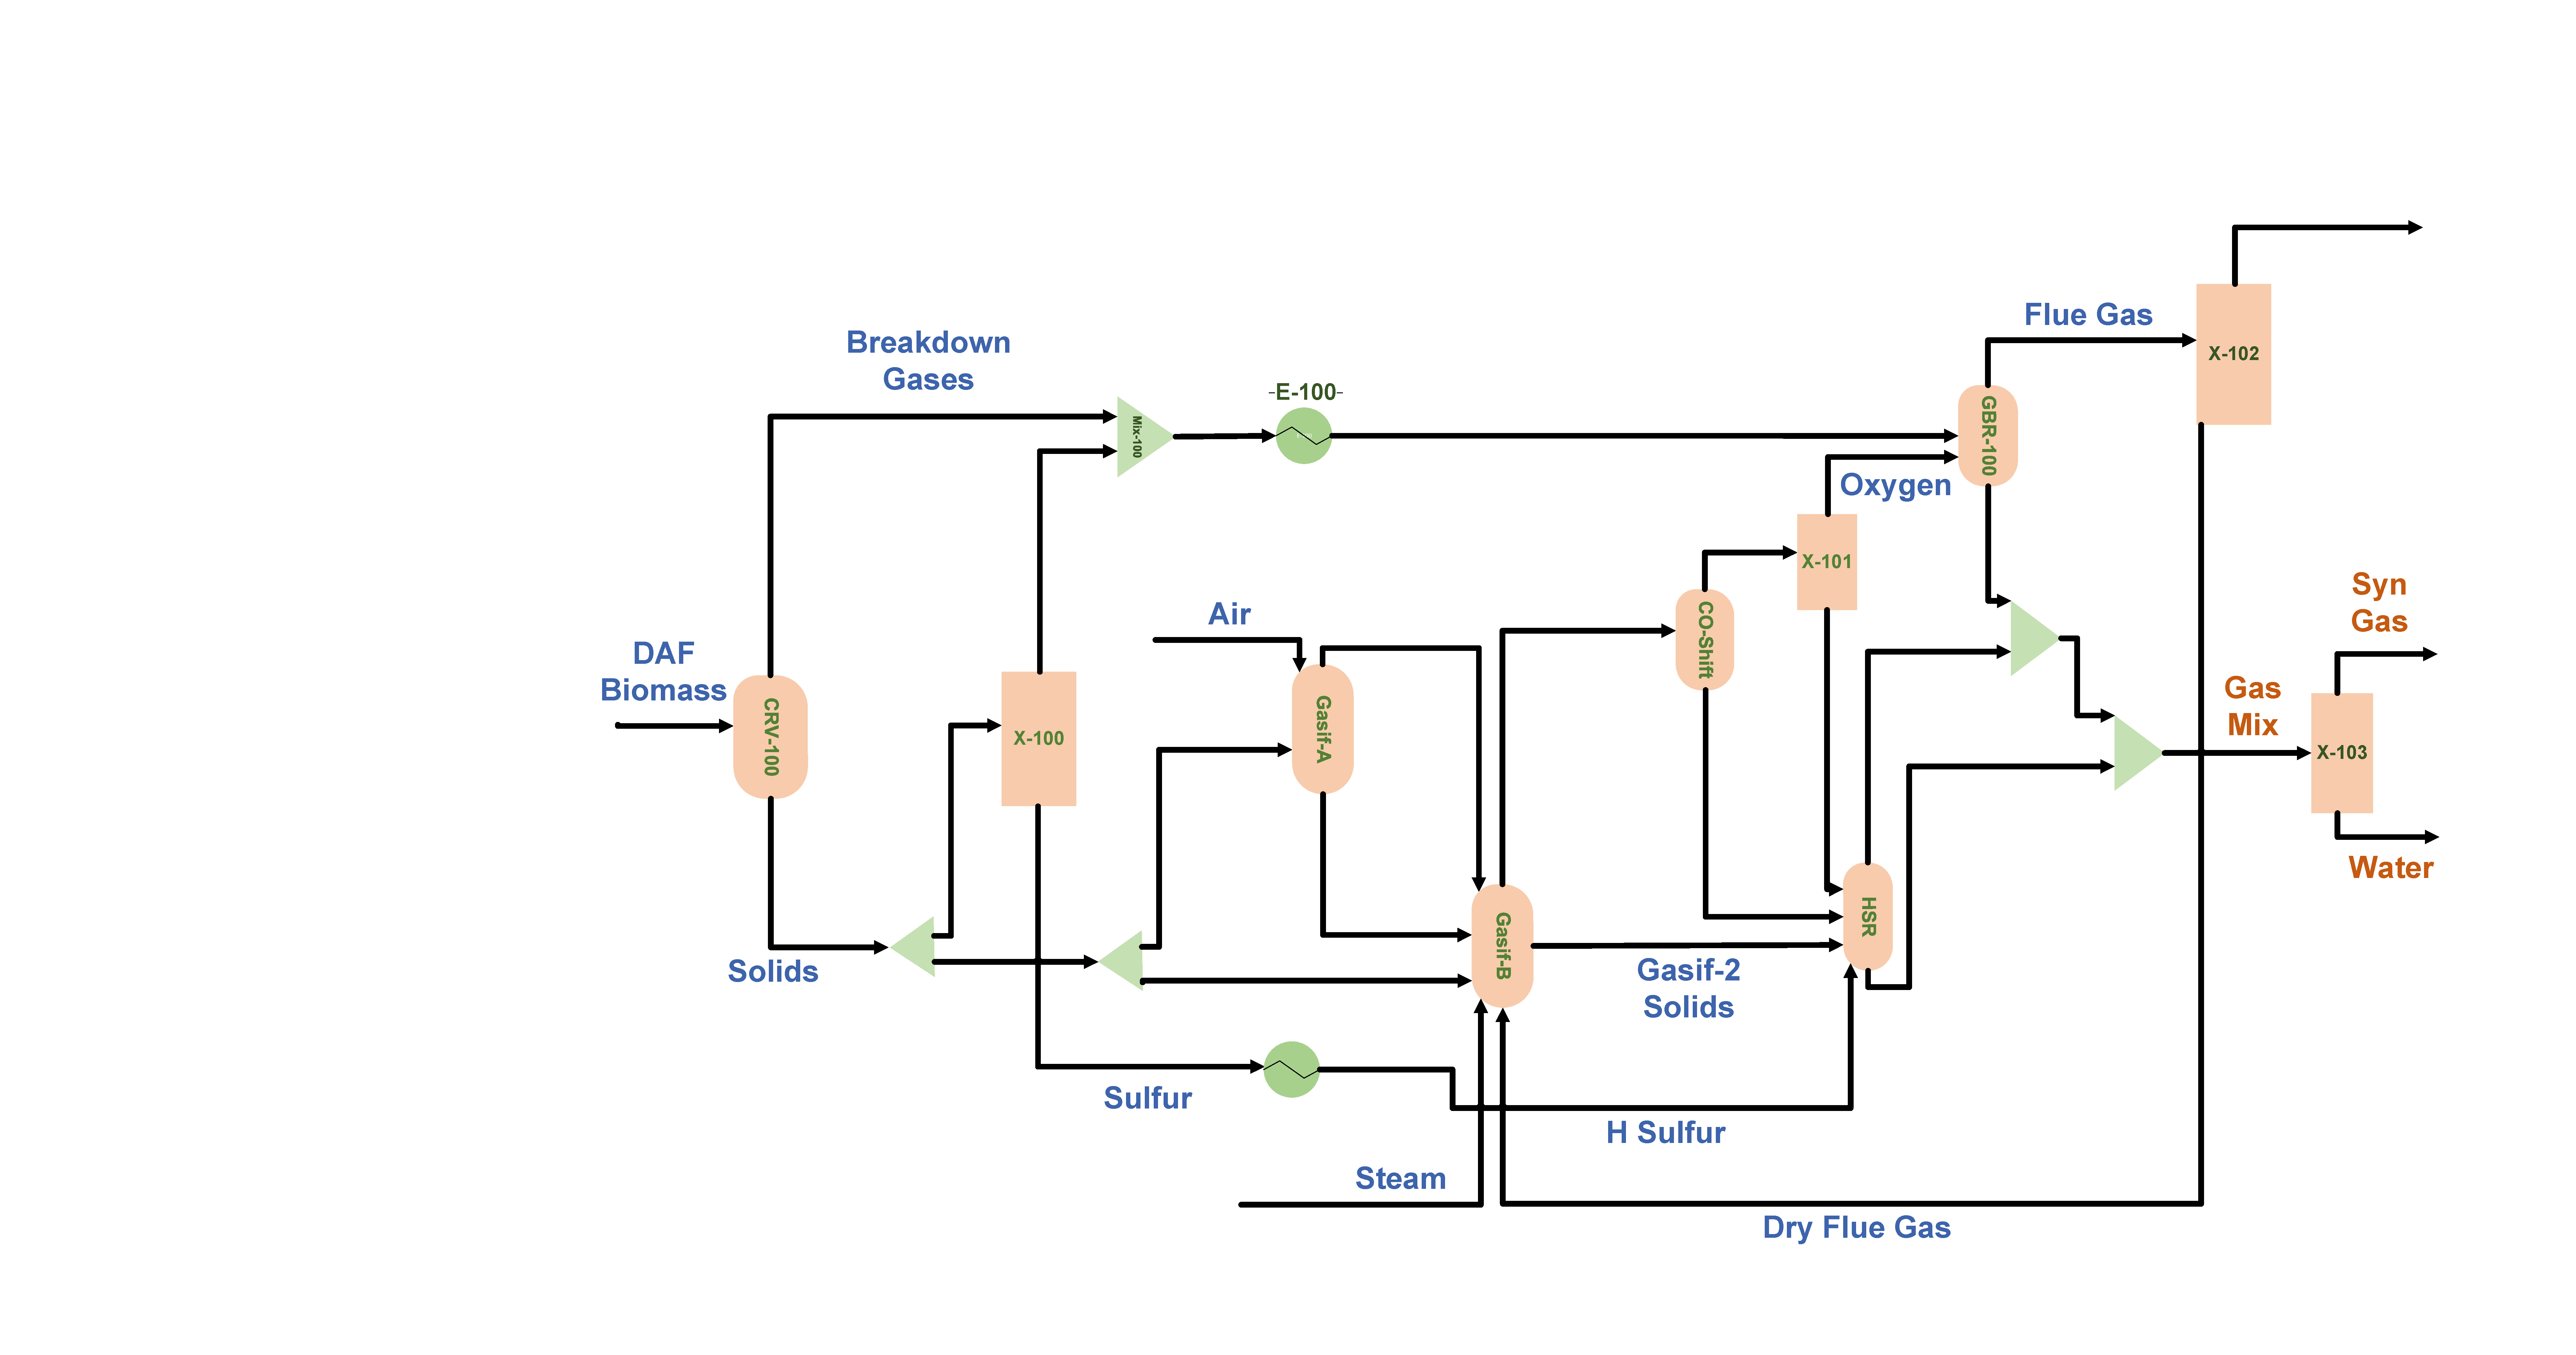
\includegraphics[width=0.98\textwidth]{figures/main/fig1_process_flowsheet.pdf}
\caption{Simplified process-flow diagram for the integrated gasification--\TSA{} feed-generation train. DAF biomass is converted in CRV-100 and split in X-100 into solid and gas-derived process streams. The staged gasification section receives the labelled air and steam inputs; downstream blocks represent CO-shift adjustment, oxygen/combustion recycle, sulfur handling, gas mixing and \add{final X-103 idealized component split into dry syngas and a separate
mixed-contaminant outlet labelled ``Water''.} The detailed Aspen HYSYS flowsheet and stream-level data are provided in Fig.~S1 and Tables~S4--S5.}
\label{fig:pfd}
\end{figure}

\begin{table}[htbp]
\centering
\caption{\add{Reaction definitions and specified conversions in the
reference (Simulation~1) and production (P-1) HYSYS configurations.
BM denotes the hypothetical biomass component. R1--R6 implement
pseudo-component decomposition; the remaining rows identify
specified conversions or Gibbs-free-energy-based equilibrium
reactions. A 0\% prescribed conversion indicates that the
specified reaction route is inactive in that model configuration,
not that the chemical pathway is physically impossible.
The reactor-modelling approach follows
\citet{Bassyouni2014DatePalmHYSYS}; the numeric conversion
settings are this study's model specifications, not published
experimental rate or conversion measurements.}}
\label{tab:reactions}
\scriptsize
\begin{adjustbox}{max width=\textwidth}
\revtableon
\begin{tabular}{cllll}
\toprule
Rxn & Reaction & Basis/type & Simulation 1 & P-1 \\
\midrule
R1 & BM $\rightarrow$ 11.102 \ce{H2O} & BM conversion & 5.47\% & 5.47\% \\
R2 & BM $\rightarrow$ 16.651 C(s) & BM conversion & 55.48\% & 55.48\% \\
R3 & BM $\rightarrow$ 99.206 \ce{H2} & BM conversion & 4.53\% & 4.53\% \\
R4 & BM $\rightarrow$ 7.140 \ce{N2} & BM conversion & 0.4686\% & 0.4686\% \\
R5 & BM $\rightarrow$ 6.237 S(s) & BM conversion & 1.015\% & 1.015\% \\
R6 & BM $\rightarrow$ 6.250 \ce{O2} & BM conversion & 33.04\% & 33.04\% \\
R7 & C + $0.5$\ce{O2} $\rightarrow$ CO & C conversion & 20\% & 0\% \\
R8 & C + \ce{O2} $\rightarrow$ \ce{CO2} & C conversion & 5\% & 5\% \\
R9 & C + \ce{CO2} $\rightarrow$ 2 CO & C conversion & 5\% & 0\% \\
R10 & CO + \ce{H2O} $\rightleftharpoons$ \ce{CO2} + \ce{H2} & equilibrium & Gibbs free energy & Gibbs free energy \\
R11 & \ce{N2} + 3\ce{H2} $\rightleftharpoons$ 2\ce{NH3} & equilibrium & Gibbs free energy & Gibbs free energy \\
R12 & S + \ce{H2} $\rightarrow$ \ce{H2S} & S conversion & 100\% & 100\% \\
R13 & C + 2\ce{H2} $\rightarrow$ \ce{CH4} & C conversion & 5\% & 5\% \\
\bottomrule
\end{tabular}
\revtableoff
\end{adjustbox}
\end{table}

Gasifier temperature (\SIrange{650}{850}{\celsius}) and \add{steam mass flow}
(\SIrange{50}{150}{kg.h^{-1}}) were swept over 20{,}301 upstream scenarios
\add{(a $101 \times 201$ grid, with steam varied from
\SI{50}{kg.h^{-1}} to \SI{150}{kg.h^{-1}} in
\SI{1}{kg.h^{-1}} steps and gasifier temperature from
\SI{650}{\celsius} to \SI{850}{\celsius} in
\SI{1}{\celsius} steps).} \add{For each upstream scenario and each adsorbent, the adsorption temperature
was held at \SI{298}{K}, while the regeneration (desorption) temperature
was varied across ten \TSA{} thermal set-points between \SI{313.2}{K}
and \SI{450}{K}. This produced 203{,}010 scoring rows per adsorbent
and 609{,}030 scoring rows in total. Throughout the manuscript,
``\TSA{} thermal set-point'' refers to the regeneration temperature,
not the adsorption temperature.}

\subsection{TSA scoring model and response metrics}
\label{sec:tsa}

The separation section is represented by an equilibrium \TSA{} scoring model
for a fixed bed packed with HKUST-1, Cu-TDPAT or Zeolite~13X. The
HYSYS-derived dry syngas composition is used as the inlet to the scoring
calculation, and material-dependent uptake and working capacity are evaluated
from the corresponding isotherm model. Because hydrogen is the weakly
adsorbed light product in this impurity-removal configuration, \Htwo{} is
treated as the raffinate product and its direct uptake is neglected in the
productivity calculation. This treatment is consistent with the much stronger
adsorption of \COtwo{}, CO and \CHfour{} on the selected adsorbents over the
relevant partial-pressure range, and with the process objective of retaining
impurities while allowing hydrogen-rich gas to pass through the bed.

For HKUST-1 and Cu-TDPAT, the single-component loading is represented by the
single-site Langmuir form,
\begin{equation}
q_i = \frac{q_i^{\mathrm{sat}} b_i p_i}{1+b_i p_i},
\label{eq:langmuir}
\end{equation}
and the mixture loading by the extended Langmuir form,
\begin{equation}
q_i = \frac{q_i^{\mathrm{sat}} b_i p_i}{1+\sum_j b_j p_j}.
\label{eq:extended}
\end{equation}
\add{The extended Langmuir form with unequal saturation capacities is used here
as a screening-level approximation for competitive uptake in the MOF
mixtures. Such models are not universally thermodynamically consistent,
and the present calculations have not been shown to reproduce the numerical
material rankings from Ideal Adsorbed Solution Theory (IAST). Accordingly,
the predicted working capacities and the Cu-TDPAT/Zeolite~13X selection
boundary are interpreted within the adopted equilibrium-model framework
\citep{Streb2020VPSAH2CO2,Streb2021Zeolite13X}.} Neglect of direct \Htwo{}
co-adsorption in the productivity calculation is consistent with standard
low-pressure hydrogen-purification screening practice, in which
impurity-adsorbent binding is much stronger than \Htwo-adsorbent binding
across the relevant partial-pressure range
\citep{Delgado2014PSAH2,Golmakani2017PSAVSATSA,Streb2020VPSAH2CO2}.

Temperature-dependent affinity parameters were fitted for HKUST-1 and
Cu-TDPAT using this form. Zeolite~13X, whose cationic aluminosilicate surface
is more heterogeneous, is represented with the temperature-dependent
Ruthven--Sips isotherm \citep{Ruthven1984PSA} using parameters from Park
et al.~\citep{Park2016Zeolite13X}, as tabulated by Streb and
Mazzotti~\citep{Streb2020VPSAH2CO2}. The Sips form reduces to the Langmuir
form in the homogeneous-surface limit; all three adsorbents are then passed
through the same downstream working-capacity, inventory and productivity
definitions. Full parameter tables, base-case stream data and supporting
isotherms are provided in the Supporting Information.

\add{The multicomponent adsorption calculations in this study were based on extended competitive
isotherm formulations to ensure a consistent and computationally tractable comparison across
the gasification--adsorption screening space. These models are established engineering
approximations, although their quantitative predictions may differ from those obtained using
thermodynamically based approaches such as IAST, particularly for mixtures with strongly
dissimilar adsorption affinities or saturation capacities. Accordingly, the predicted working
capacities, productivity values, and exact position of the Cu-TDPAT/Zeolite 13X crossover should
be regarded as model-dependent. Importantly, the central finding of this work concerns the
coupling between gasification conditions, the resulting impurity composition, and adsorbent
selection, rather than a universal numerical crossover boundary. The reported material-
selection regions therefore provide a comparative equilibrium-screening basis for identifying
promising process--adsorbent combinations, while definitive quantitative rankings require
further validation using multicomponent adsorption data or more rigorous equilibrium and
cyclic models.}

The \TSA{} score uses a common four-step interpretation: adsorption,
purge/blowdown, heating/desorption and cooling/re-equilibration. The cycle
time is standardised to $t_{\mathrm{cycle}}=\SI{900}{s}$, corresponding to
15\,min or 0.25\,h; this basis follows comparative \PSA/VSA/\TSA{}
hydrogen-purification simulations reported by Golmakani et al.\
\citep{Golmakani2017PSAVSATSA}. Specific hydrogen productivity is defined as
\begin{equation}
\Pi_{\Htwo}=\frac{n_{\Htwo,\mathrm{out}}}{m_{\mathrm{ads}}\,t_{\mathrm{cycle}}},
\label{eq:prod}
\end{equation}
where $n_{\Htwo,\mathrm{out}}$ is the moles of hydrogen exiting during the
productive adsorption step, $m_{\mathrm{ads}}$ is the dry adsorbent mass and
$t_{\mathrm{cycle}}=\SI{900}{s}$.

The impurity-specific adsorbent mass requirement is
\begin{equation}
m_{\mathrm{ads},i}=\frac{n_{i,\mathrm{feed}}\,\eta_i}{\Delta q_i},
\label{eq:mass}
\end{equation}
where $\eta_i$ is the prescribed removal factor and $\Delta q_i$ is the
working capacity over the swing window. The controlling inventory is
$m_{\mathrm{ads,max}}=\max_i(m_{\mathrm{ads},i})$ with
$i\in\{\COtwo,\mathrm{CO},\CHfour\}$. The present scoring uses
$\eta_i=0.99$ for each retained impurity, so the model sizes the adsorbent
inventory required to meet a common removal target. Product purity and
hydrogen recovery are constrained only indirectly through this common removal
target; they are not independently optimised outputs of the equilibrium
scoring model.

Specific regeneration energy includes sensible heating of the bed,
adsorbent and adsorbed phase, together with the heat associated with
desorbing the retained impurities. The explicit form of the regeneration
energy calculation is given as Eq.~S7 in the Supporting Information. All
inventory-normalised quantities are reported on an adsorbent-mass basis so
that HKUST-1, Cu-TDPAT and Zeolite~13X are compared under the same
normalisation. Where inherited figure-axis labels use ``MOF'' as shorthand,
the corresponding quantity is the adsorbent-mass-normalised value.

\add{The adsorption and regeneration temperature definitions, working-capacity
calculation, controlling adsorbent inventory, hydrogen-productivity
normalisation and regeneration-energy calculation are specified in
Section~3 of the Supporting Information (Eqs.~S4--S7). The corresponding
isotherm, adsorption-enthalpy and heat-capacity parameters are given
in Tables~S6--S10. The impurity removal target is 99\% for each retained
impurity, adsorption pressure is \SI{1}{bar}, and the common cycle time
is \SI{900}{s}.}

A pressure-swing variant of the same equilibrium scoring logic is reported
as a robustness check in the Supporting Information. In that table, adsorption
pressure is fixed at \SI{1}{bar} and the desorption endpoint is swept from
\SIrange{0.01}{0.63}{bar}. The pressure-swing results are used only to test
whether the adsorbent-ranking partition is preserved when the swing variable
changes from temperature to pressure. Because the spreadsheet score does
not include full compressor or vacuum-system work, the pressure-swing variant
is used only as a ranking-robustness check and should not be read as a full
PSA/VSA energy comparison.

\subsection{Tree-ensemble surrogate and feature attribution}
\label{sec:surrogate}

A tree-ensemble surrogate provides a compact attribution layer over the
computed process--material scoring table. Its role is to reproduce the
computed response surface using controllable variables and adsorbent
identity, then quantify which inputs contribute most strongly to each
screening output. The surrogate serves as an interpretability tool over
the computed atlas, not as an independent predictor of unstudied
adsorbents.

The surrogate inputs were steam mass flow, gasifier temperature, \TSA{}
thermal set-point and one-hot adsorbent identity. Syngas mole fractions and
product molar flow were deliberately excluded because they are outputs of
the gasifier simulation and therefore mediate the relation between gasifier
set-points and adsorption performance. Including both gasifier set-points
and their downstream composition consequences would mix upstream causes with
intermediate variables and make attribution ambiguous. Composition variables
are therefore analysed directly in the gasifier maps, while surrogate
attribution is restricted to controllable process/material variables.

Separate XGBoost regressors were trained for five outputs: adsorbent mass
controlled by \CHfour{}, adsorbent mass controlled by CO, adsorbent mass
controlled by \COtwo{}, hydrogen productivity and regeneration energy.
Performance was evaluated under both a random row split and a
gasifier-scenario-grouped split, in which all rows associated with a
held-out gasifier scenario were excluded from training. TreeSHAP is used
for feature attribution because it accommodates the categorical
adsorbent-identity input and the interactions between controllable
variables in a single unified framework; equivalent attribution through
analytical partial derivatives of the scoring equations would require
enumerating pairwise adsorbent comparisons and interaction terms
case-by-case. Exact TreeSHAP values were then computed for the trained
tree ensembles to quantify the mean contribution of each controllable
input to each output. Architecture, hyperparameters, split definitions,
held-out metrics and parity plots are reported in Section~S8 of the
Supporting Information. Under the more conservative gasifier-scenario-grouped
split, the surrogate gives $R^2>0.96$ for all five outputs, supporting its use
as a high-fidelity attribution layer over the computed atlas rather than as an
extrapolative model for unstudied materials.


\section{Results and discussion}
\label{sec:results}

\subsection{Adsorbent ranking is a function of gasifier set-points}
\label{sec:ranking}

\Cref{fig:winner} is the organizing result of the study. For each of the
20{,}301 gasifier scenarios in the steam-feed/gasifier-temperature grid, the
hydrogen-productivity score was first averaged over the ten \TSA{} thermal
set-points for each adsorbent. The adsorbent with the highest average score was
then assigned as the winner for that gasifier state. This construction removes
the arbitrariness of discussing one selected operating point and asks instead
whether the preferred adsorbent changes across the upstream process window. The
answer is a clear two-region partition of the gasifier operating space
(\Cref{fig:winner}a). Cu-TDPAT gives the highest productivity score in a
low-steam, moderate-temperature region covering approximately 23\% of the
\add{gasifier scenarios (4{,}640 of 20{,}301), whereas Zeolite~13X gives the highest}
score across the remaining 77\%, which spans higher steam feed, higher gasifier
temperature, or both. HKUST-1 does not appear as a productivity winner in the
winner map, consistent with its lower-throughput, lower-energy role discussed in
\Cref{sec:tradeoff,sec:cdf,sec:mass}.

\add{The quantitative selection boundaries reported here are specific to the
investigated configuration, comprising pine sawdust gasification, a fixed
adsorption pressure of \SI{1}{bar}, and an assumed pretreated, dry syngas
feed. Different feedstocks, adsorption pressures, or feed-conditioning
conditions may shift these boundaries; the broader conclusion concerns the
dependence of adsorbent selection on upstream gasification conditions rather
than the universality of the reported 23\%/77\% partition.}

\add{The original productivity winner map (Fig.~2a) is a temperature-averaged screening comparison, not an operating strategy: each scenario selects the material with the highest mean productivity over the ten saved TSA thermal set-points. We also compared materials at each common fixed set-point and after maximizing productivity over these same ten set-points independently for each material and scenario. These comparisons use only the existing TSA results.}

\begin{figure}[htbp]
\centering
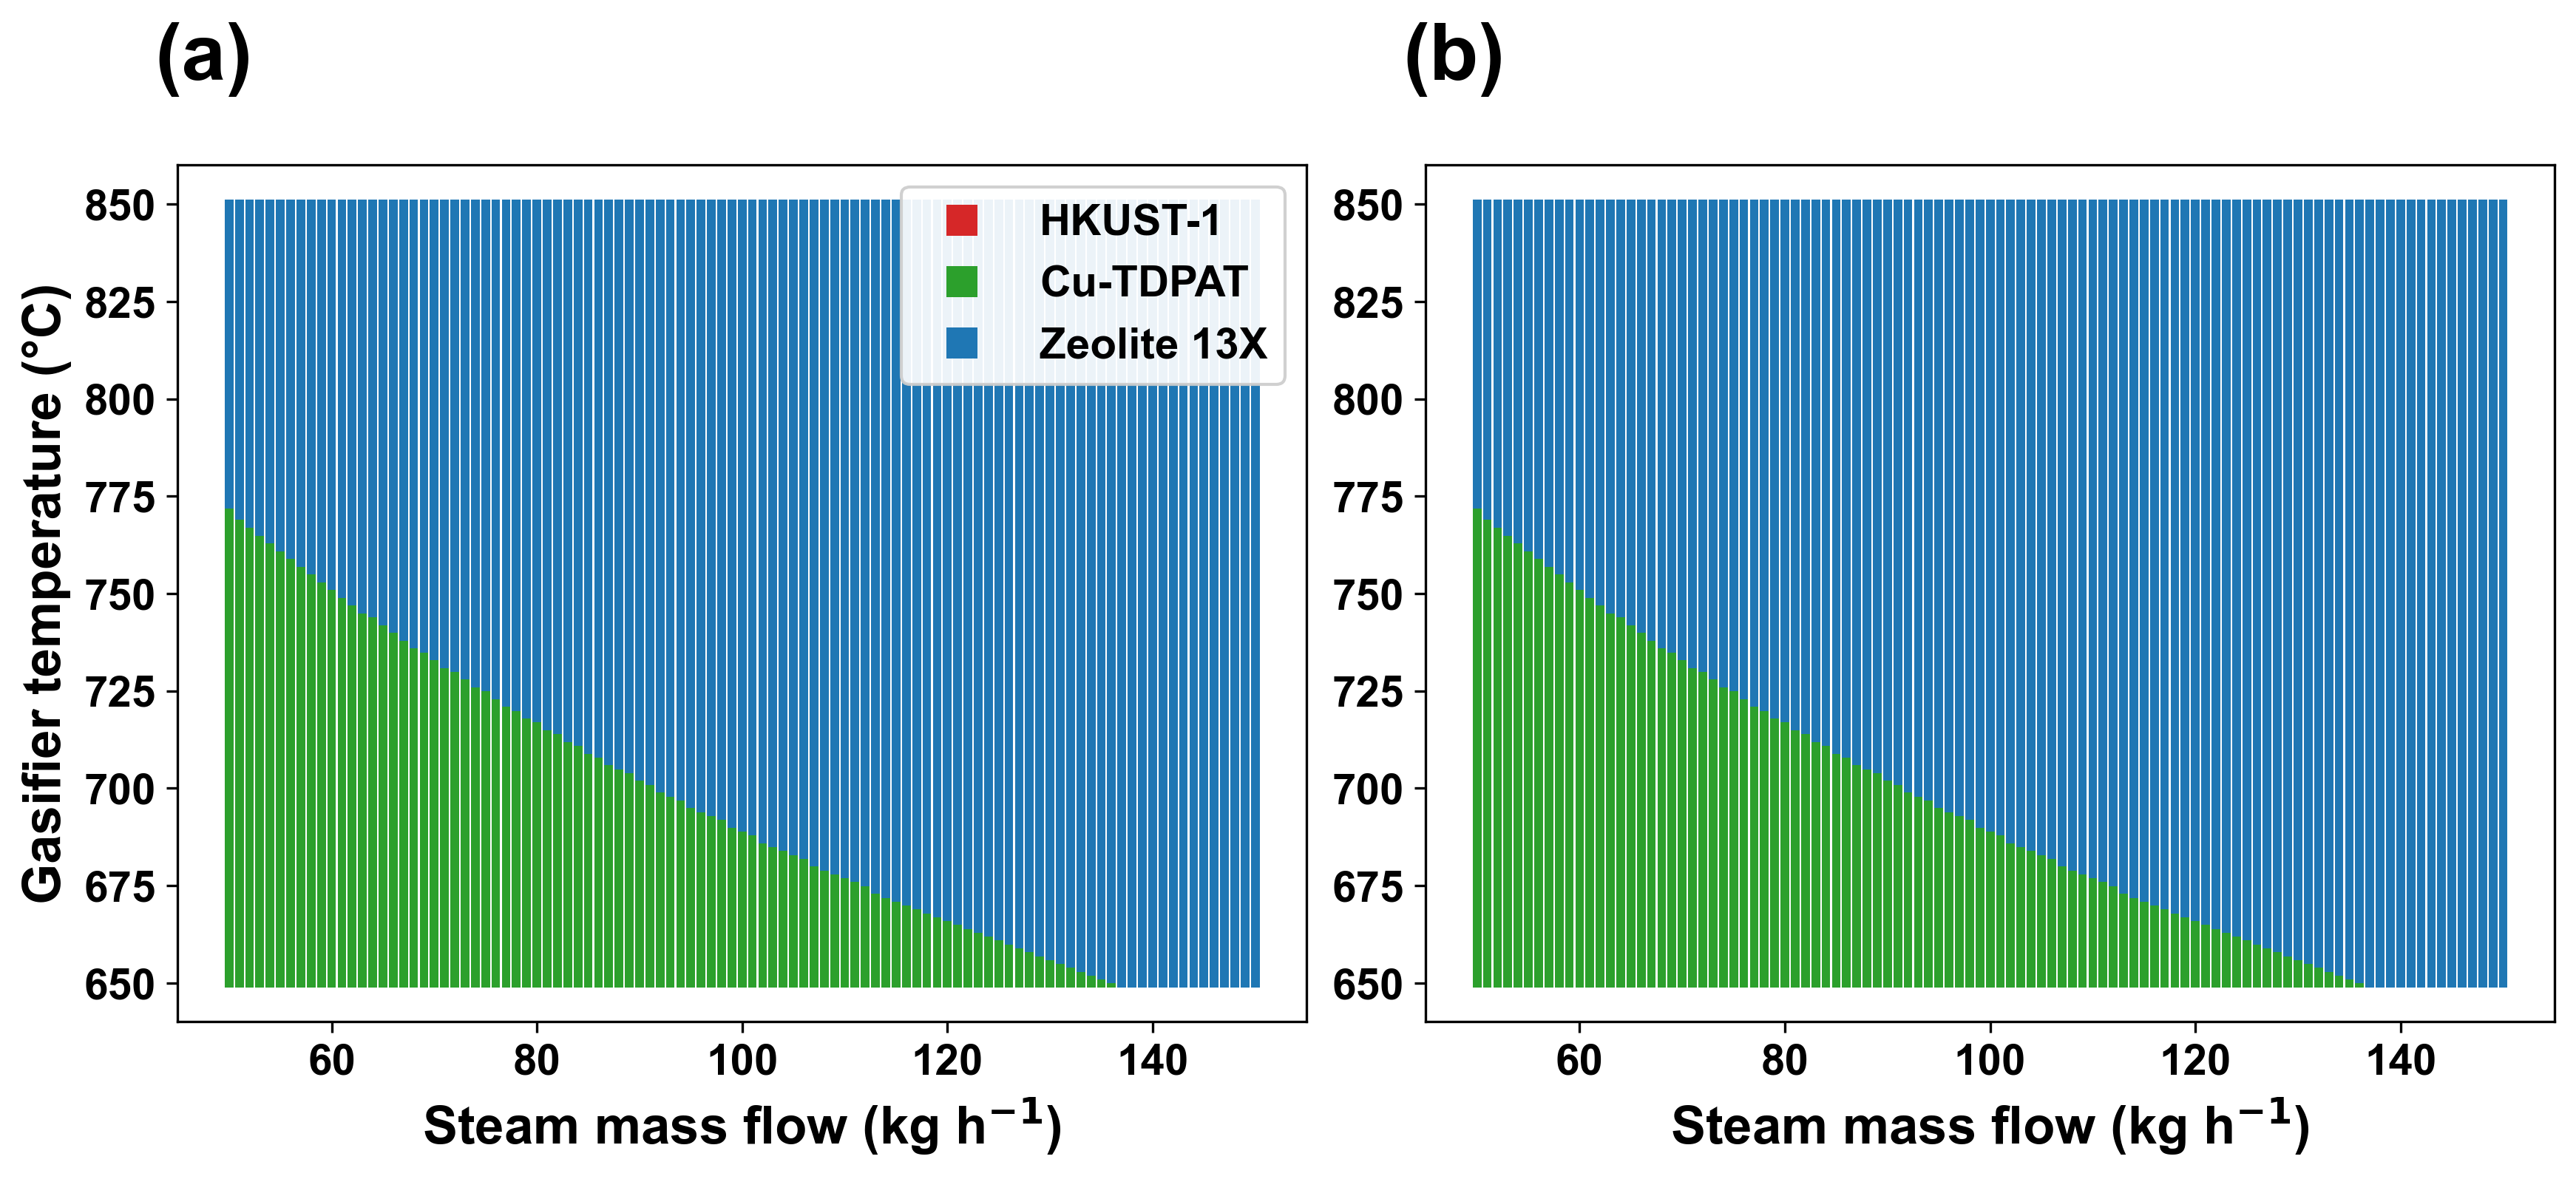
\includegraphics[width=0.95\textwidth]{../outputs/figures/main/fig2_winner_map.png}
\caption{Adsorbent ranking across the gasifier operating space. For each of
the 20{,}301 gasifier scenarios (steam mass flow $\times$ gasifier temperature)
the adsorbent with the highest hydrogen productivity averaged over the ten
\TSA{} thermal set-points is identified.
(a) Winner by hydrogen productivity, $\Pi_{\Htwo}$.
(b) Winner by productivity per unit regeneration energy, $\Pi_{\Htwo}/E_{\mathrm{reg}}$.
A smooth boundary separates a Cu-TDPAT-preferred region (low steam, moderate
temperature, \num{\approx 23}\% of scenarios) from a Zeolite~13X-preferred
region (\num{\approx 77}\% of scenarios). HKUST-1 does not appear as a winner
under either metric. The two partitions are essentially identical, indicating
that the crossover is not an artefact of the choice of ranking metric.}
\label{fig:winner}
\end{figure}

\add{The temperature-averaged map assigns 4,640 of 20,301 scenarios to Cu-TDPAT (22.8560\%), 15,661 to Zeolite 13X (77.1440\%) and none to HKUST-1. Each of the ten fixed TSA thermal set-points from 313.2 to 450.0~K gives exactly these proportions (the minimum and maximum coincide for each material), with 0\% of scenario winners changed at every set-point. Individually optimized set-points give the same proportions and change 0 of 20,301 winners (0\%; Fig.~S19). The original temperature-averaged screening map is therefore retained.}

The boundary between the two regions is smooth rather than scattered or
checkerboarded. It runs from approximately (\SI{50}{kg.h^{-1}},
\SI{775}{\celsius}) to (\SI{140}{kg.h^{-1}}, \SI{650}{\celsius}), and it is
preserved when the ranking metric is changed from hydrogen productivity to
productivity per unit regeneration energy (\Cref{fig:winner}b). This behaviour
is important because it separates a physically interpretable crossover from a
numerical artefact. If the winner map were controlled mainly by a single metric
choice or by isolated outlier scenarios, the productivity and productivity-per-energy
maps would not be expected to share the same boundary. Instead, the same
gasifier states that favour Cu-TDPAT by productivity also favour it after
regeneration energy is included, while the remaining states favour Zeolite~13X.
Within the equilibrium scoring basis used here, the ranking therefore reflects
the way the gasifier changes the impurity hierarchy delivered to the bed.

\add{The visually smooth boundary in the gasifier operating plane does not imply
near-equal productivity scores on either side. Across the 20{,}301 gasifier
scenarios and ten fixed regeneration-temperature set-points (203{,}010
comparisons), the winning adsorbent exceeds the runner-up in hydrogen
productivity by at least 18.96\% (relative to the runner-up), with no
margins below 5\%. In the saved equilibrium-screening inputs, the sharp
change in preferred material coincides with zero-valued \CHfour{} mole
fractions and a corresponding change in the impurity controlling the
required adsorbent inventory. The plotted boundary is therefore a
model-based selection partition rather than a resolved near-tie; its
physical location and uncertainty cannot be established without propagating
feed-composition and isotherm uncertainties.}

The partition is also analytically invariant to the two most arbitrary
normalisation choices in the scoring model: the imposed impurity-removal factor
$\eta_i$ and the cycle time $t_{\mathrm{cycle}}$. Uniform scaling of $\eta_i$
over the range 0.90 to 0.999, non-uniform scaling to industrially motivated
targets (99.99\% CO removal, 99\% CO$_2$ removal, 95\% CH$_4$ removal), and
cycle-time scaling from 600 s to 1500 s all give identical winner-map shares
(22.86\% Cu-TDPAT, 77.14\% Zeolite~13X). This invariance follows directly from
the structure of Eqs.~S3--S6: when $\eta_i$ or $t_{\mathrm{cycle}}$ scales the
three adsorbents on the same basis, inventory-normalised productivity scales
uniformly and the ranking within a given scenario is preserved. The sensitivity
therefore shows that the winner-map partition is not created by the chosen
removal target or cycle-time normalisation. It should not be interpreted as a
validation of the gasification chemistry assumptions themselves; those
assumptions define the feed-composition family that is subsequently scored. A
full sensitivity table and visualisation of the winner maps under non-uniform
removal targets are provided in Section~S12 of the Supporting Information.

A pressure-swing variant of the same equilibrium scoring rule gives the same
practical message without being promoted to a separate process comparison. In
that check, adsorption is fixed at \SI{1}{bar} and the desorption endpoint is
swept from \SIrange{0.01}{0.63}{bar} (Section~S11 and Fig.~S17 of the
Supporting Information). The winner shares remain essentially unchanged:
Cu-TDPAT wins \num{22.86}\% of scenarios and Zeolite~13X wins \num{77.14}\%,
compared with \num{22.90}\% and \num{77.10}\% under the temperature-swing
score. This result is used only to show that the ranking boundary is not tied
to the thermal swing variable. It is not a full \PSA{}/VSA energy comparison,
because compressor and vacuum-system work are outside the pressure-swing score.

The remainder of Section~\ref{sec:results} explains why the boundary appears
where it does. \Cref{sec:syngas} shows how gasifier set-points reshape the dry
syngas composition and hence the impurity hierarchy delivered to the bed.
\Cref{sec:tradeoff} connects that hierarchy to energy--productivity envelopes
for the three adsorbents. \Cref{sec:cdf} checks whether the crossover persists
at the distribution level rather than only at selected points. \Cref{sec:shap}
uses the tree-ensemble surrogate to attribute the screening outputs to
controllable process/material variables. \Cref{sec:mass} introduces inventory
as a secondary selection criterion, and \Cref{sec:rules} converts the figures
into process-conditioned selection observations.

\subsection{Gasifier set-points define the impurity regime that the bed must solve}
\label{sec:syngas}

\Cref{fig:syngas} shows the process origin of the winner map. The gasifier does
not only set the hydrogen fraction; it also determines which impurity the
adsorbent must retain most effectively and regenerate most economically. In
panel~(a), the \Htwo{} fraction rises toward the high-temperature region,
consistent with endothermic steam gasification, reforming and biomass-cracking
chemistry. Panel~(b) shows the accompanying \COtwo{} enrichment as steam
promotes water--gas-shift chemistry. Panel~(c) shows that \CHfour{} is
suppressed across most of the grid and survives mainly in the lower-temperature,
lower-steam corner where methanation is less strongly penalised. Panel~(d) shows
CO highest in the low-steam, high-temperature region and reduced when additional
steam shifts CO toward \COtwo{} and \Htwo. The corresponding one-variable
sensitivity plots are reported in the SI (Figs.~S2--S5), and the base-case
composition is tabulated in Tables~S4--S5. These trends are consistent with
recent Aspen-based biomass-gasification studies showing that gasifier
temperature, steam-to-biomass ratio, equivalence ratio and downstream
shift/capture configuration reshape the hydrogen-rich syngas composition
delivered to the separation section
\citep{Rosha2023MSWGasificationMEA,Matta2024OlivePomaceAspen}.

\begin{figure}[htbp]
\centering
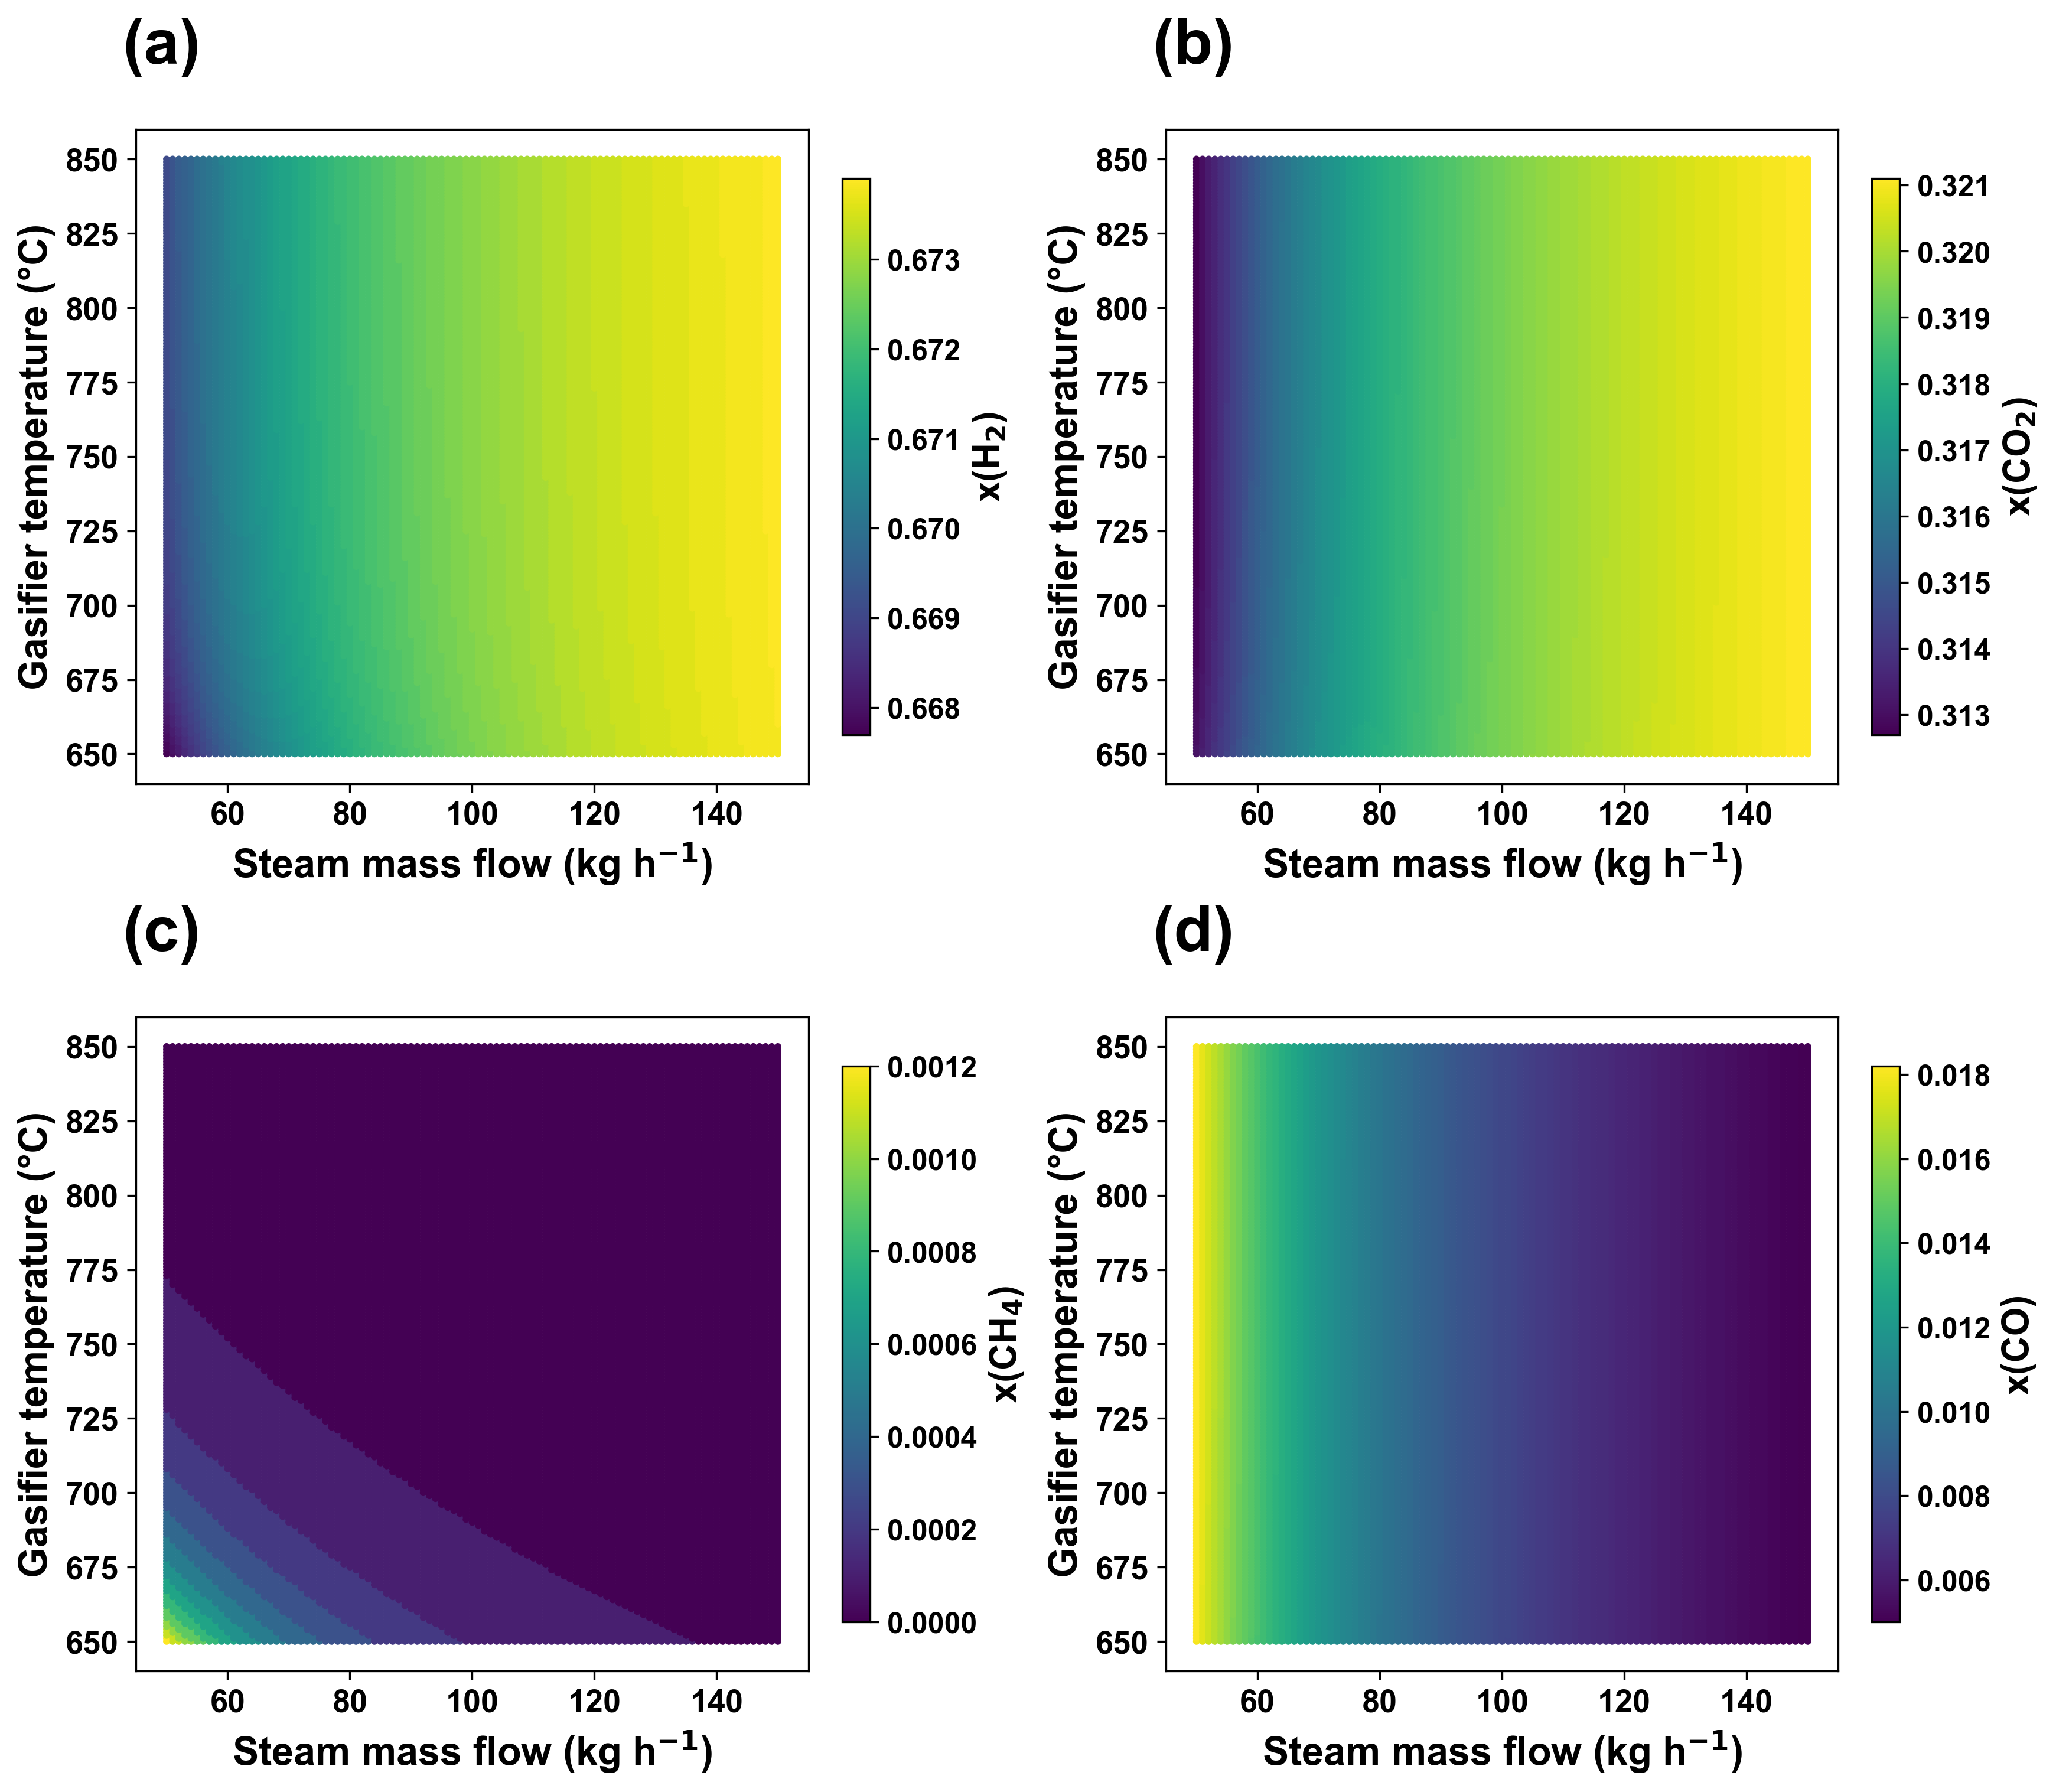
\includegraphics[width=0.65\textwidth]{../outputs/figures/main/fig3_syngas_composition_maps.png}
\caption{Gasifier operating conditions define the impurity regime delivered
to \TSA{}. Panels show the dry syngas mole fractions of (a) \Htwo, (b) \COtwo,
(c) \CHfour{} and (d) CO as functions of gasifier temperature and steam feed.
Steam simultaneously suppresses CO and \CHfour{} while enriching \COtwo{}, so
upstream steam optimisation changes not only hydrogen yield but also the
impurity that limits the downstream adsorbent.}
\label{fig:syngas}
\end{figure}

Three regimes are therefore visible in the gasifier plane: a CO-influenced
high-temperature/low-steam region, a \COtwo-rich high-steam region, and a
methane-influenced low-temperature/low-steam corner. They are not equivalent
from the viewpoint of adsorbent selection. \COtwo{} mainly increases
regeneration duty and adsorbent inventory because it is the most strongly
adsorbed impurity across much of the atlas. CO is present at lower mole
fraction but can become important because its interaction with open-metal sites
and zeolite cation sites can change the limiting inventory. \CHfour{} is smaller
again, but it becomes relevant when the feed enters the low-steam corner where
pore size, hydrophobicity and weakly polar adsorption environments determine
whether methane is retained or displaced. This explains why the methane-rich
corner of \Cref{fig:syngas}c aligns with the Cu-TDPAT-preferred region in
\Cref{fig:winner}a, whereas the \COtwo-rich and CO-influenced regions align with
Zeolite~13X. Adsorbent selection cannot therefore be treated as a downstream
choice made after fixing one nominal syngas composition: the upstream gasifier
creates the impurity problem that the adsorbent ranking is solving.

\subsection{Energy--productivity envelopes explain the partition mechanistically}
\label{sec:tradeoff}

\Cref{fig:tradeoff} translates the winner-map boundary into an
energy--productivity trade-off. The x-axis is useful hydrogen throughput per
unit adsorbent inventory, and the y-axis is the thermal penalty required to
desorb the retained impurities. A favourable material is therefore not simply
the material with the largest equilibrium uptake. It is the material that
combines enough working capacity with a regeneration penalty that does not erase
the productivity gain.

Cu-TDPAT (panels a,b) reaches the high-productivity envelope under
methane-limited operation when the \TSA{} thermal set-point provides sufficient
working-capacity leverage. This is the same part of the gasifier plane where
\CHfour{} survives in the feed, and it is the regime where Cu-TDPAT's pore
architecture can translate into a favourable inventory-normalised score
\citep{Wu2012CuTDPAT,Liu2014CuTDPAT,Asgari2021CuTDPAT}. Under CO-limited
operation, the Cu-TDPAT envelope is more restricted because CO and \COtwo{}
increase the retained impurity burden and narrow the useful thermal window.
HKUST-1 (panels c,d) occupies a lower-productivity but lower-energy region. For
an open-Cu framework with strong \COtwo{} interactions, moisture sensitivity and
site competition, this is better interpreted as a low-duty or polishing window
than as a bulk high-throughput role
\citep{Abid2023HKUST,Yin2018HKUSTCO,Zelenka2022HKUSTAmine,Rostom2024CuBTC}.

\add{As a practical indication of the moisture limitation, experimental
water-vapour exposure of HKUST-1 at \SI{50}{\celsius} preserved its
characteristic crystalline structure at 70\% relative humidity but
led to structural collapse at 90\% relative humidity
\citep{AlJanabi2015HKUSTWater}.
This reported failure range is not an allowable moisture threshold for
the present \SI{298}{K} adsorption step: water can compete for open Cu
sites before structural collapse, so the proposed polishing role assumes
effective upstream drying and would require cyclic-stability verification
\citep{AlJanabi2015HKUSTWater,Doman2019HKUSTWater}.}
Zeolite~13X (panels e,f) provides the most robust global envelope, especially
under CO-limited operation, consistent with its established role in
multicomponent impurity removal and layered-bed hydrogen purification
\citep{Streb2021Zeolite13X,Delgado2014PSAH2,Yang2025Layered13X}.

\begin{figure}[htbp]
\centering
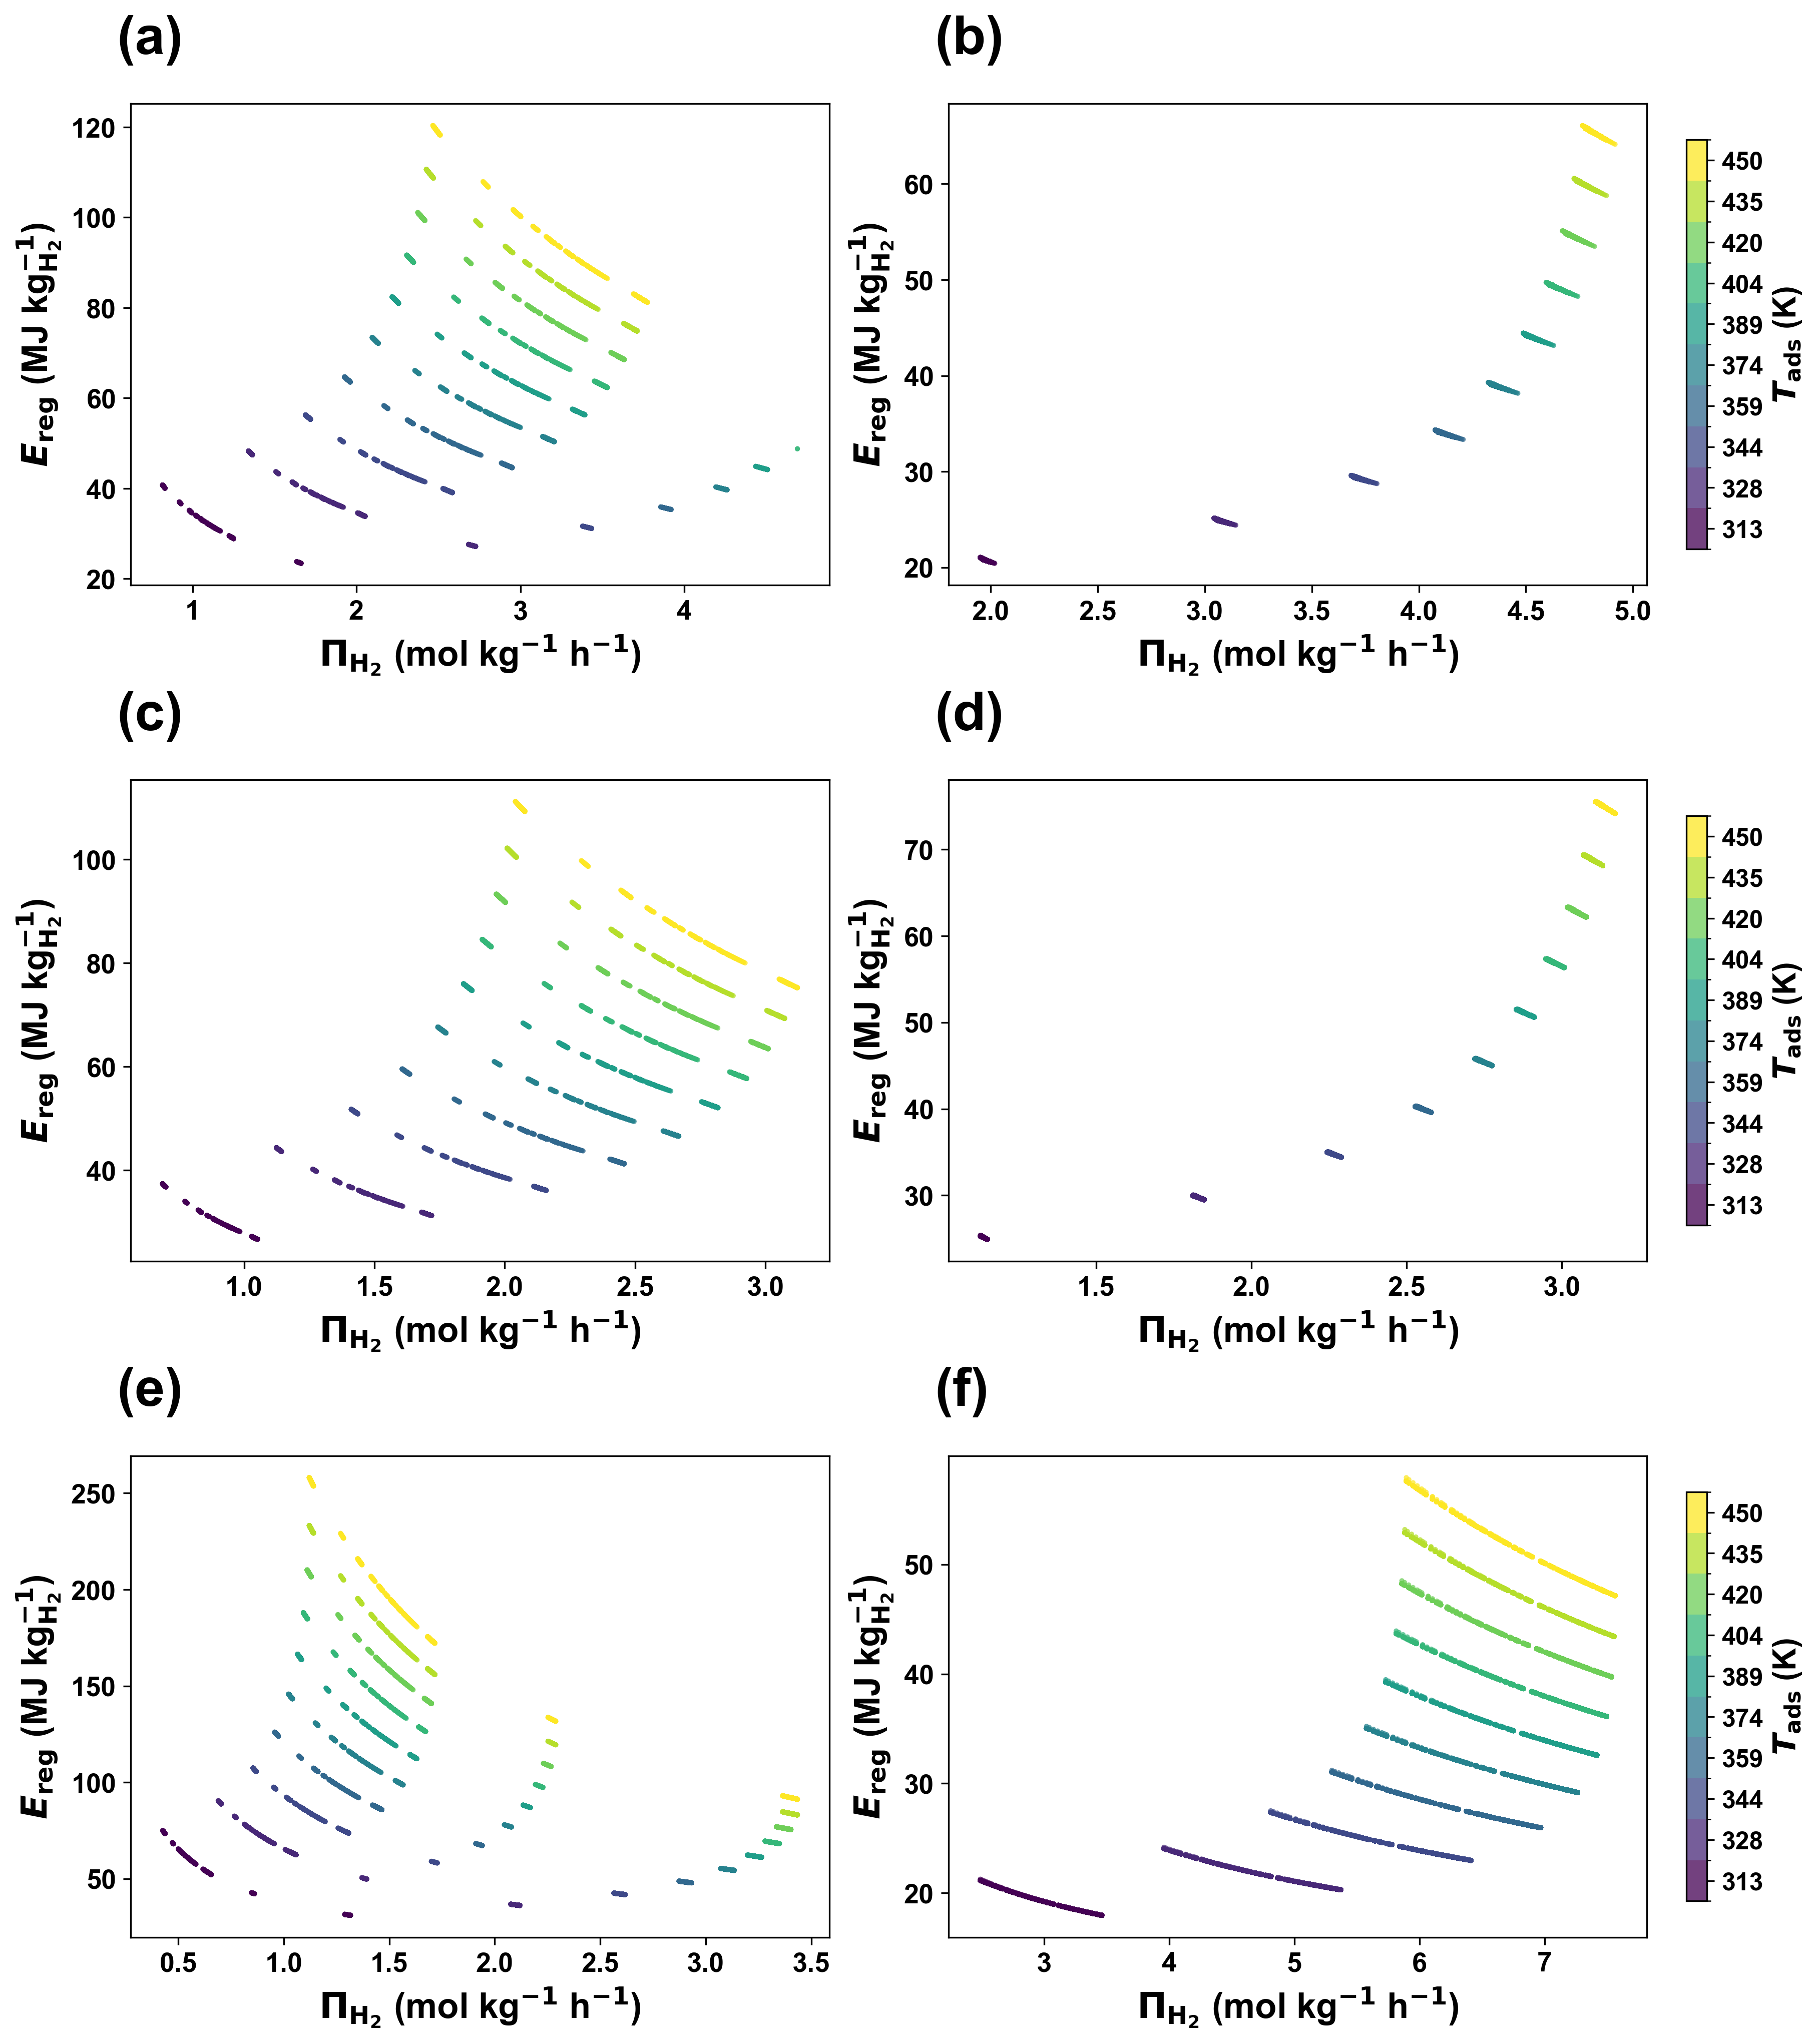
\includegraphics[width=0.82\textwidth]{../outputs/figures/main/fig4_energy_productivity_tradeoff.png}
\caption{Energy--productivity envelopes for the three adsorbents. Panels
(a,b) show Cu-TDPAT under (a) methane-limited and (b) CO-limited operation;
panels (c,d) show HKUST-1 under (c) methane-limited and (d) CO-limited
operation; panels (e,f) show Zeolite~13X under (e) methane-limited and (f)
CO-limited operation. Colour indicates the \TSA{} thermal set-point. Within this screening score, Zeolite~13X gives the most robust global
envelope, Cu-TDPAT approaches the high-productivity envelope under
methane-influenced/temperature-flexible conditions and HKUST-1 occupies a
lower-energy niche.}
\label{fig:tradeoff}
\end{figure}

The figure also clarifies why the result should be framed as regime-dependent
rather than as a universal MOF--zeolite ranking. Zeolite~13X is the safest
benchmark when the feed is broadly variable or CO/\COtwo{}-dominated. Cu-TDPAT
is competitive only when the feed and swing temperature align with the impurity
it handles most favourably. HKUST-1 is not a productivity winner but marks a
low-duty region that may matter in polishing or staged-bed concepts. Together
with \Cref{fig:winner,fig:syngas}, this establishes the mechanistic chain:
gasifier set-points fix the impurity hierarchy; the impurity hierarchy fixes
the limiting inventory for each adsorbent; the limiting inventory fixes the
regeneration penalty relative to throughput; and that penalty determines which
adsorbent lies at the favourable end of its envelope. The winner map in
\Cref{fig:winner} is the projection of this chain onto the gasifier operating
plane.

\subsection{Cumulative-distribution ranking confirms the crossover}
\label{sec:cdf}

Point comparisons can hide how often a material actually occupies a favourable
regime. \Cref{fig:cdf} therefore reports empirical cumulative distributions of
$\Pi_{\Htwo}$ across the atlas under \CHfour-limited and CO-limited operation.
The CDF representation is useful here because it does not depend on kernel
bandwidth choices and directly shows percentile-level performance. At any
cumulative fraction, the rightmost curve identifies the adsorbent with the
higher typical productivity at that percentile.

\begin{figure}[htbp]
\centering
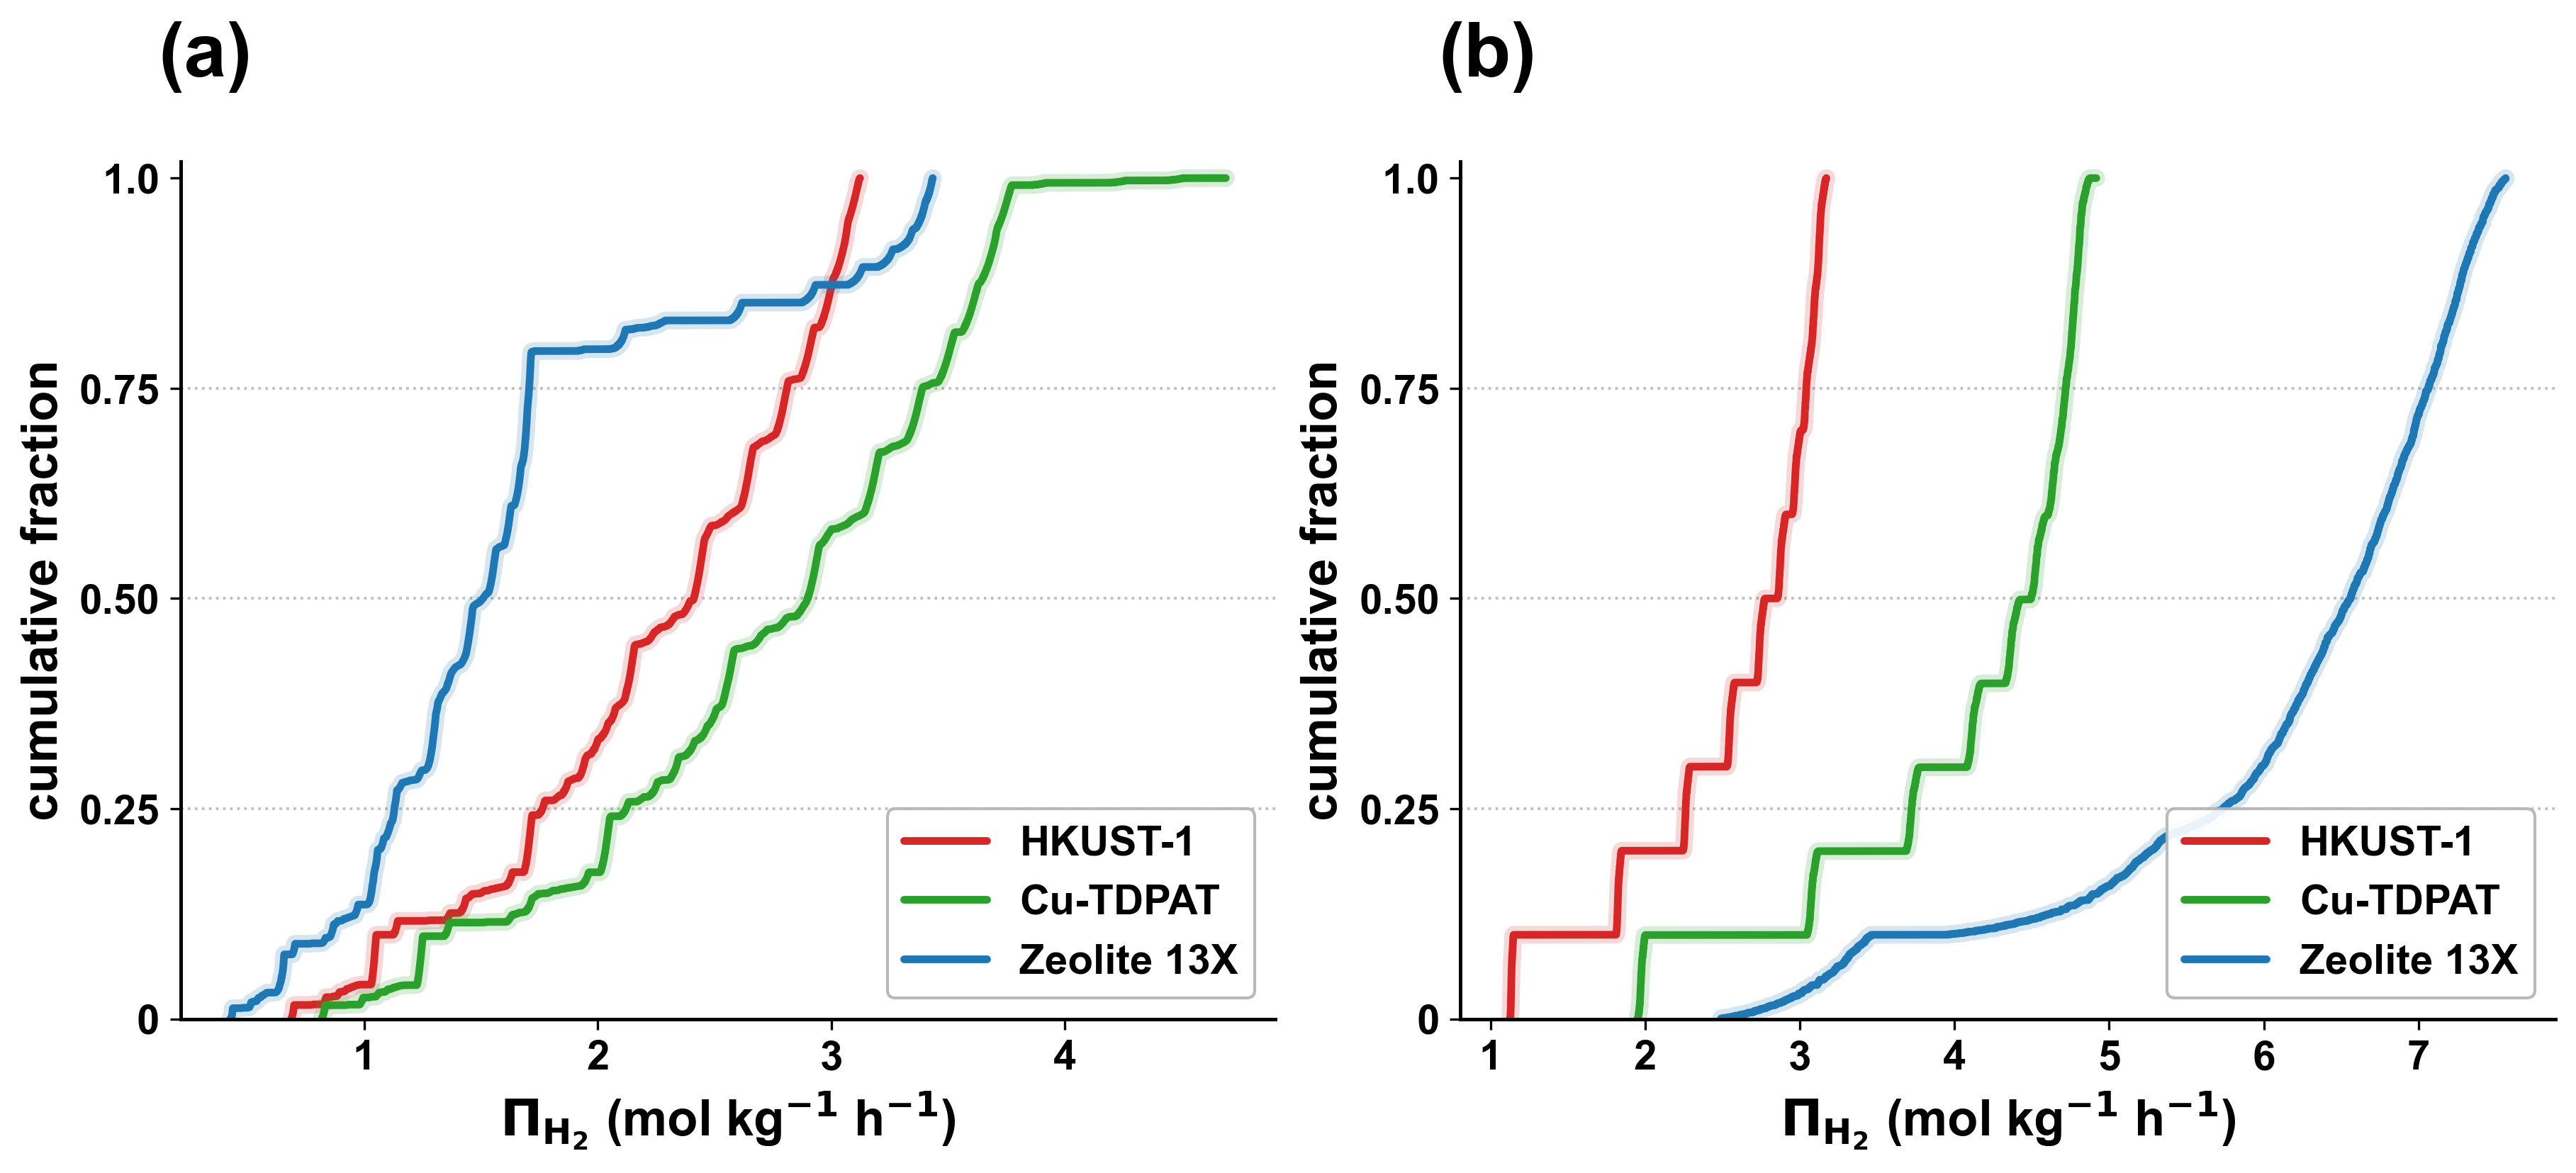
\includegraphics[width=0.90\textwidth]{../outputs/figures/main/fig5_productivity_distributions.png}
\caption{Empirical cumulative distributions of adsorbent-mass-normalised
hydrogen productivity, $\Pi_{\Htwo}$, across the atlas.
(a) \CHfour-limited operation. (b) CO-limited operation. Each curve
shows the fraction of scenarios reaching productivity at or below the
plotted value; the rightmost curve at any given cumulative fraction
identifies the adsorbent with the higher typical productivity at that
percentile. In (a), Zeolite~13X saturates near
\SI{1.8}{mol.kg^{-1}.h^{-1}}: approximately 80\% of its scenarios
lie at or below that value, while Cu-TDPAT and HKUST-1 extend into
higher productivity bands. In (b), the three adsorbents occupy
near-non-overlapping productivity ranges. Zeolite~13X spans roughly
\SIrange{2.5}{7.5}{mol.kg^{-1}.h^{-1}}, Cu-TDPAT spans
\SIrange{2}{5}{mol.kg^{-1}.h^{-1}} and HKUST-1 spans
\SIrange{1}{3}{mol.kg^{-1}.h^{-1}}, giving a clear ranking
within the CO-limited subset. Dotted horizontal lines mark the
25th, 50th and 75th percentiles. Step-shaped features reflect the ten
discrete \TSA{} thermal set-points spanned in the atlas.}
\label{fig:cdf}
\end{figure}

Under \CHfour-limited operation (panel~a), Zeolite~13X reaches a productivity
ceiling near \SI{1.8}{mol.kg^{-1}.h^{-1}}, where roughly 80\% of its scenarios
accumulate. HKUST-1 and Cu-TDPAT continue to higher screening productivities,
and Cu-TDPAT extends furthest to the right. This is the specific and limited
sense in which MOFs become competitive in the present atlas: in
methane-influenced feeds, their equilibrium working-capacity score can access a
higher inventory-normalised productivity band than the zeolite score. This is a
ranking result under a common screening basis, not a claim of universal MOF
superiority or of guaranteed final product-gas purity.

Under CO-limited operation (panel~b), the three distributions are almost
non-overlapping. Zeolite~13X spans roughly
\SIrange{2.5}{7.5}{mol.kg^{-1}.h^{-1}}, Cu-TDPAT spans
\SIrange{2}{5}{mol.kg^{-1}.h^{-1}}, and HKUST-1 spans
\SIrange{1}{3}{mol.kg^{-1}.h^{-1}}. The ordering is therefore clear within
this regime: Zeolite~13X $>$ Cu-TDPAT $>$ HKUST-1. This distribution explains
why Zeolite~13X occupies most of the gasifier operating plane, while the
methane-limited distribution explains why the low-steam crossover region
exists. The CDFs therefore provide a distribution-level check on the winner map:
\Cref{fig:winner} is not only a map of isolated optima, but a projection of two
separable productivity populations onto the gasifier operating plane.

\subsection{Attribution over controllable variables shows why the ranking is regime-dependent}
\label{sec:shap}

The tree-ensemble surrogate reproduces the computed scoring atlas across all
five screening outputs under a gasifier-scenario-grouped held-out test, with
$R^2 > 0.96$ on the three outputs that involve working-capacity--impurity-flow
interactions ($m_{\mathrm{ads},\CHfour}$, $\Pi_{\Htwo}$, $E_{\mathrm{reg}}$) and
$R^2 > 0.9999$ on the two outputs that are essentially deterministic algebraic
functions of the four inputs at nearly constant impurity flows
($m_{\mathrm{ads},\mathrm{CO}}$, $m_{\mathrm{ads},\COtwo}$). The surrogate is a
high-fidelity compression of the atlas over controllable variables. It is used
as a sensitivity-summarization layer rather than as an extrapolative model for
new adsorbents: exact TreeSHAP contributions give a compact view of which
process/material levers shape each screening output. Full held-out metrics and
attribution tables are provided in Section~S8 of the Supporting Information.

\add{Local derivatives of individual isotherm or working-capacity equations
describe sensitivities at a specified state, whereas the complete
gasifier--adsorption mapping also includes material-dependent responses
and switches in the controlling impurity through
$m_{\mathrm{ads,max}}=\max_i(m_{\mathrm{ads},i})$ across operating scenarios.
The XGBoost/TreeSHAP layer complements that analytical description by
summarising, over the sampled operating envelope, which controllable
inputs contribute most to each computed screening output; these surrogate
attributions are neither independent validation of the equilibrium model
nor causal effects.}

\begin{figure}[htbp]
\centering
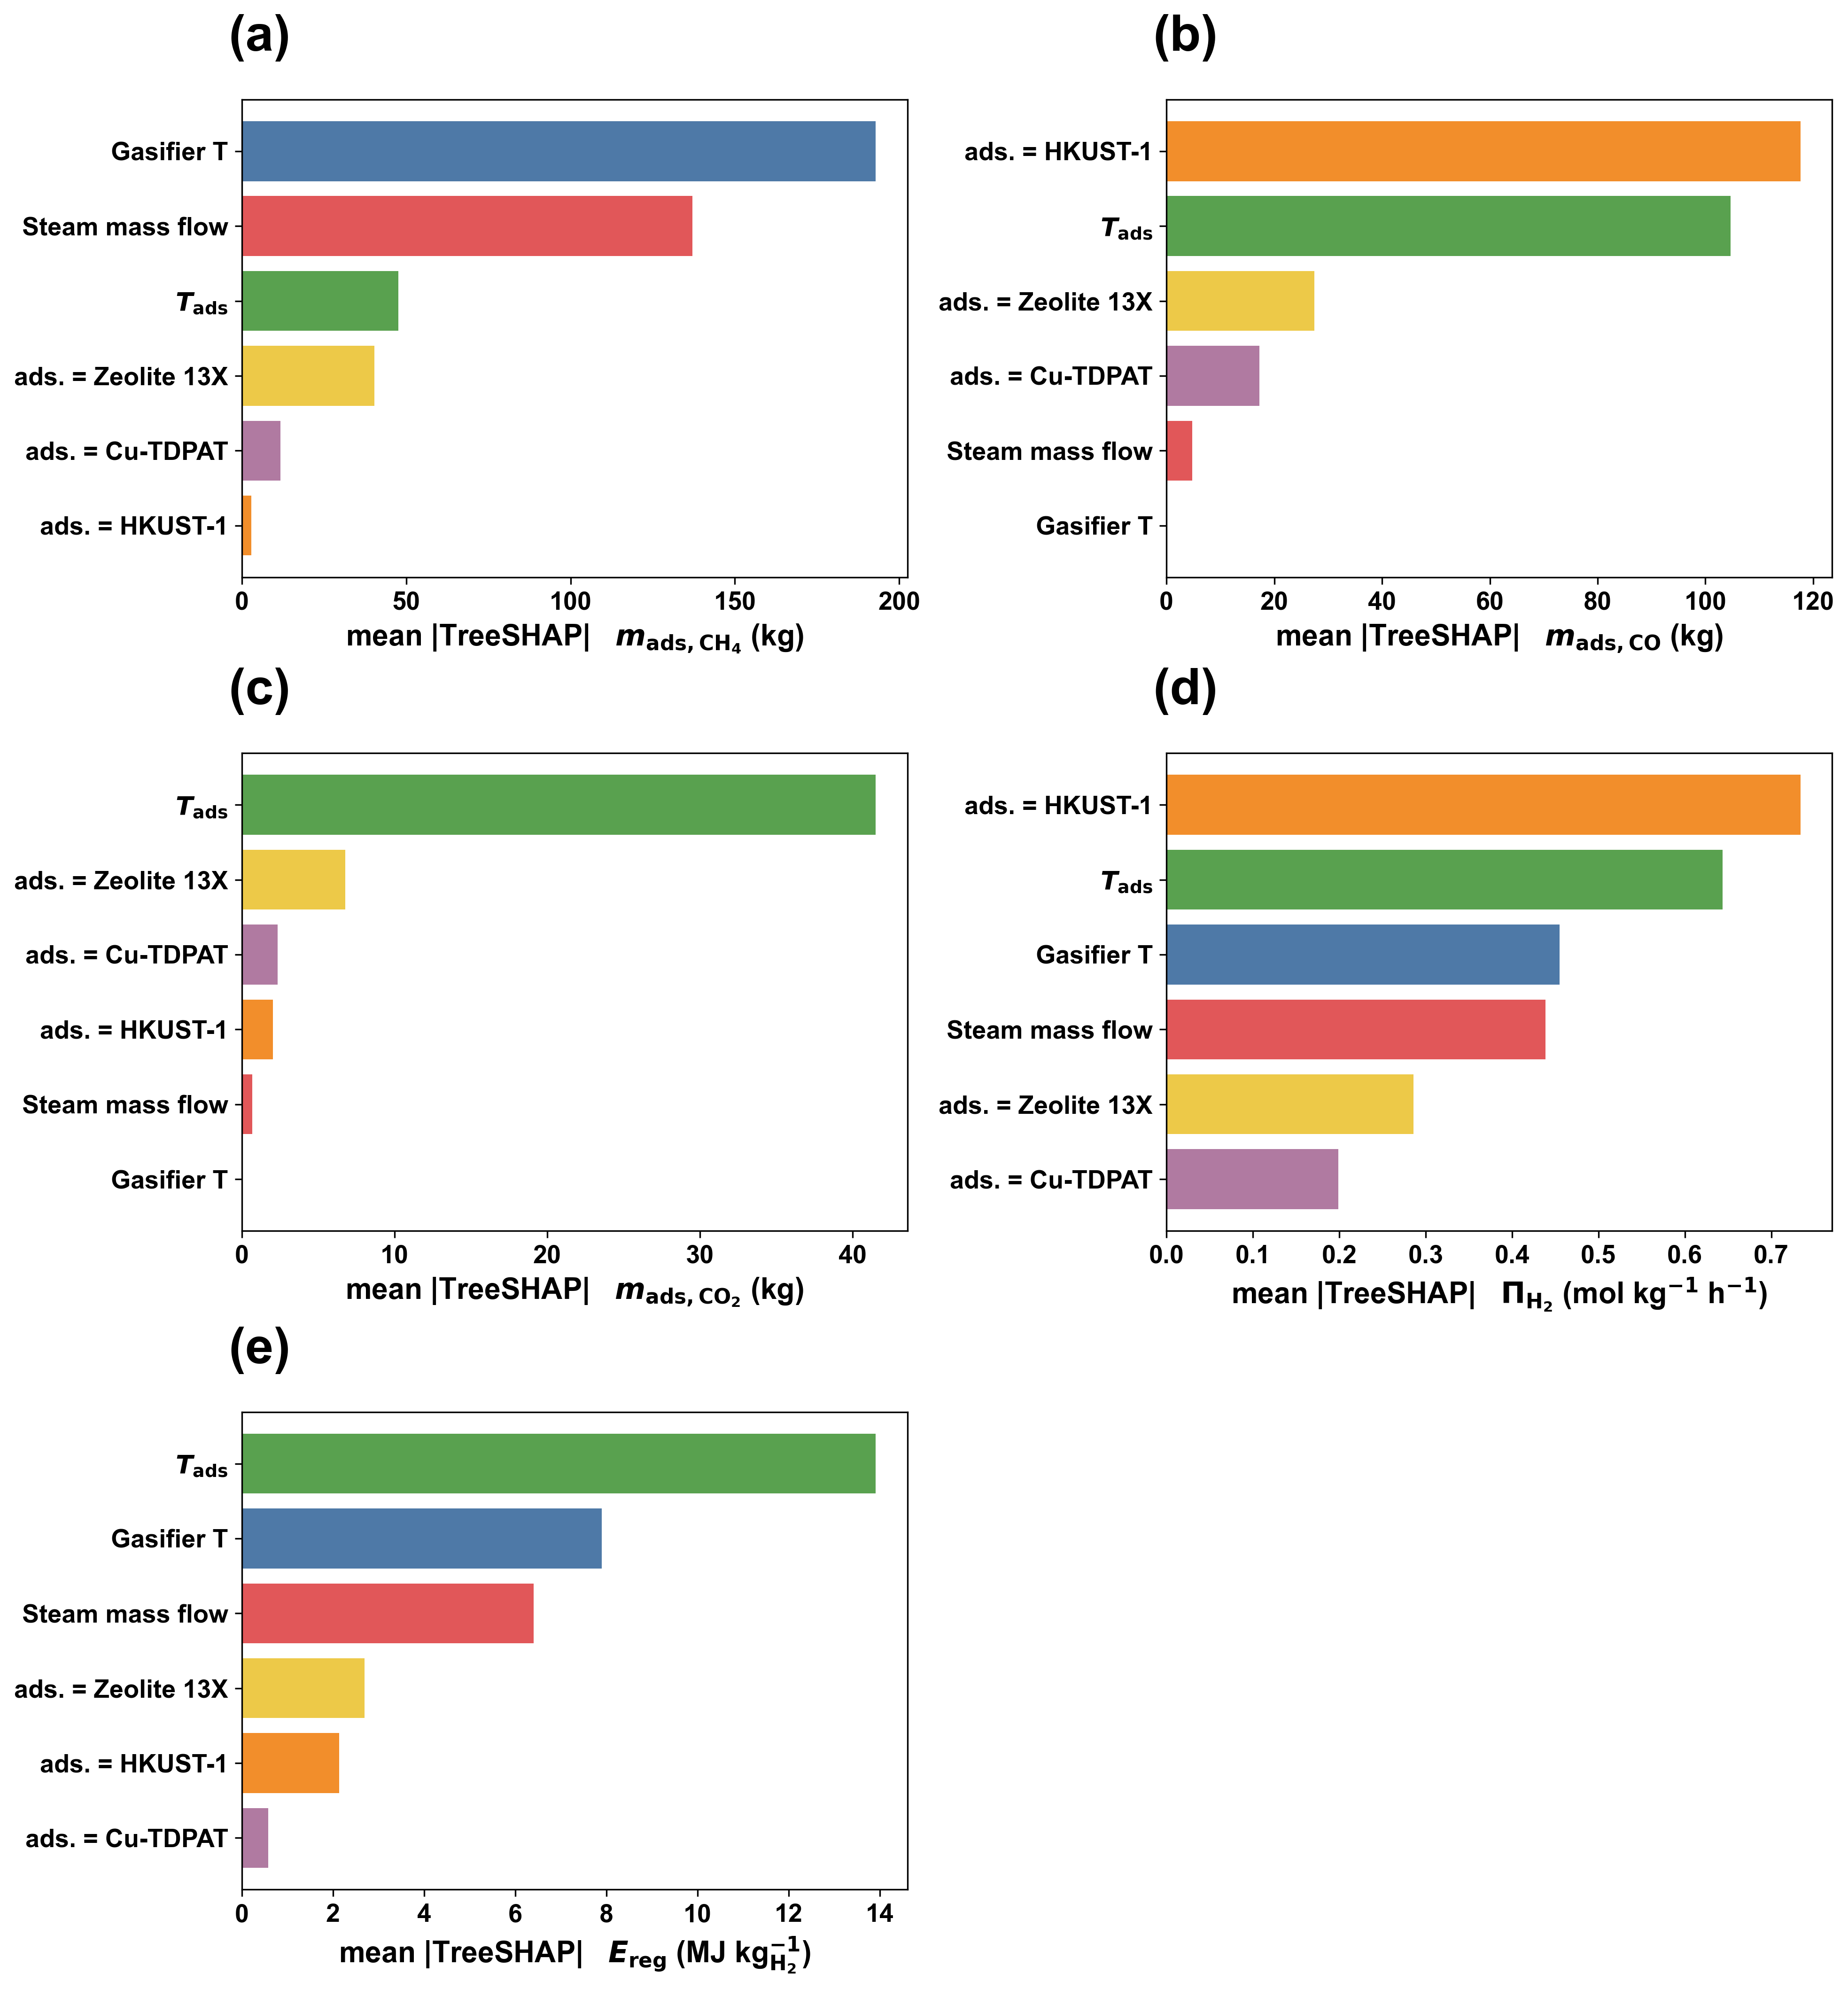
\includegraphics[width=0.98\textwidth]{../outputs/figures/main/fig6_treeshap_grouped.png}
\caption{Exact TreeSHAP attribution for the tree-ensemble surrogate trained
on controllable variables only under the gasifier-scenario-grouped split.
Bars report mean absolute TreeSHAP contribution to each of the five screening
outputs: adsorbent mass controlled by \CHfour{}, adsorbent mass controlled by
CO, adsorbent mass controlled by \COtwo{}, hydrogen productivity and
regeneration energy. CH$_4$-driven inventory is dominated by upstream
gasifier set-points; CO-driven inventory by adsorbent identity and \TSA{}
thermal set-point; \COtwo-driven inventory by the \TSA{} thermal set-point;
hydrogen productivity by a combination of all four; and regeneration energy
by \TSA{} thermal set-point with upstream contributions. This distributed
control structure is the process-level explanation for the regime-dependent
adsorbent ranking in \Cref{fig:winner}.}
\label{fig:shap}
\end{figure}

\Cref{fig:shap} shows that the ranking is not governed by one universal lever.
Methane-driven inventory is controlled mainly by upstream gasifier set-points,
consistent with methane content being set by gasification chemistry rather than
by adsorbent identity alone. CO-driven inventory is controlled by both
adsorbent identity and the \TSA{} thermal set-point, showing that CO management
depends on material chemistry as well as the regeneration window. \COtwo-driven
inventory is dominated by the \TSA{} thermal set-point, consistent with
\COtwo{} being the primary heat-regeneration burden. Hydrogen productivity is
distributed across all four levers, while regeneration energy is dominated by
the thermal set-point with additional upstream contributions.

This distributed control structure provides a quantitative link between the
figures. In the low-steam, moderate-temperature corner where methane content is
highest, the CH$_4$-driven inventory becomes more important and the score
favours Cu-TDPAT. In higher-steam or higher-temperature regions, CO and
\COtwo{} become the more important constraints; CO inventory and regeneration
energy then favour Zeolite~13X. The attribution therefore supports the same
mechanism inferred from the process maps and distributions. It does not replace
physical interpretation, but it makes the interpretation auditable by decomposing
each screening output into contributions from variables that a process/material
designer can actually choose.

\subsection{Adsorbent inventory adds a secondary selection criterion}
\label{sec:mass}

\Cref{fig:mass} examines how specific productivity changes with the controlling
adsorbent inventory, $m_{\mathrm{ads,max}}$. Because productivity is normalised
by adsorbent mass, a decline with increasing inventory is expected when
additional bed mass does not produce a proportional increase in useful hydrogen
throughput. Cu-TDPAT (panel~a) declines smoothly over its plotted range, so it
can remain competitive when footprint, adsorbent inventory or thermal-management
constraints become important. HKUST-1 (panel~b) is lower-throughput but also
comparatively smooth, consistent with its role as a low-duty or polishing
candidate. Zeolite~13X (panel~c) starts from the highest productivity region but
loses productivity more rapidly as required inventory increases.

\begin{figure}[htbp]
\centering
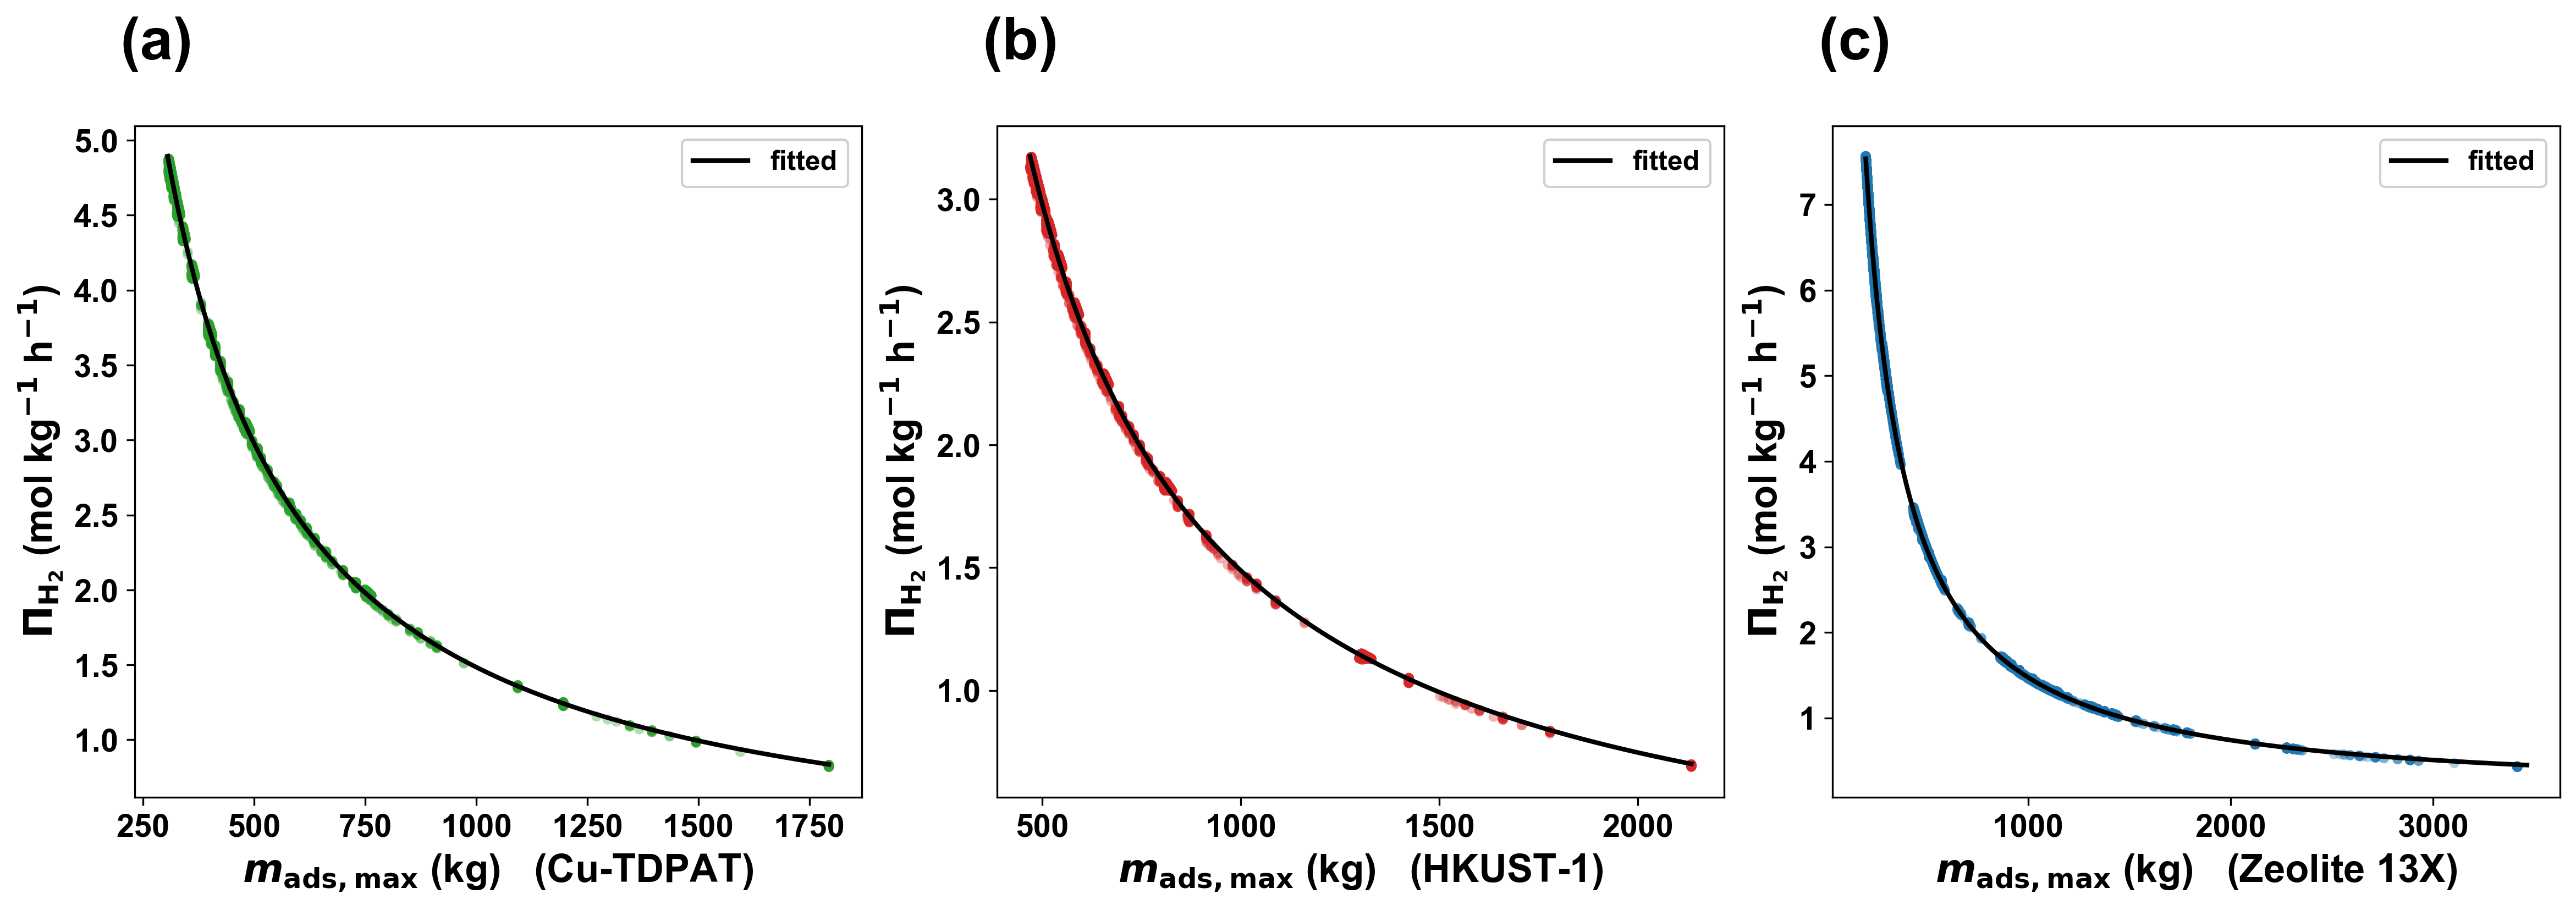
\includegraphics[width=0.90\textwidth]{../outputs/figures/main/fig7_adsorbent_mass_scaling.png}
\caption{Inventory scaling of adsorbent-mass-normalised hydrogen productivity.
Fitted curves show $\Pi_{\Htwo}$ as a function of the maximum required
adsorbent mass, $m_{\mathrm{ads,max}}$, for (a) Cu-TDPAT, (b) HKUST-1 and
(c) Zeolite~13X. Cu-TDPAT declines more smoothly than Zeolite~13X, so a MOF can become
a higher-priority screening candidate under bed-inventory or footprint
constraints even when the zeolite has the higher maximum productivity score.}
\label{fig:mass}
\end{figure}

Maximum productivity and inventory-scaled productivity are therefore different
screening criteria. This panel is not a bed-design calculation: it does not
resolve pressure drop, heat-transfer fronts or column geometry. It asks a
narrower question---whether the productivity score remains favourable after
normalisation by the adsorbent inventory required to control the limiting
impurity. On that basis, Zeolite~13X is the natural benchmark at the highest
productivity points, while MOF candidates can remain relevant when inventory,
footprint or thermal-management constraints are prioritised. \Cref{fig:mass} is
therefore complementary to \Cref{fig:tradeoff}: \Cref{fig:tradeoff} identifies
favourable operating windows in energy--productivity space, whereas
\Cref{fig:mass} asks whether performance remains attractive after the adsorbent
mass required to control the limiting impurity is included.

The thermodynamic basis for these trends is in the Supporting Information. The
individual isotherm and working-capacity panels are shown in Figs.~S6--S13, and
the composite interpretation panel is Fig.~S14. Across these data, \COtwo{}
dominates equilibrium uptake and working capacity, while CO and \CHfour{} have
much smaller absolute loadings at low pressure. This is why \COtwo{} often
controls regeneration energy, while CO and \CHfour{} can still alter ranking by
changing competitive site occupation and the identity of the limiting impurity.
The practical materials implication is that the most useful MOFs are not simply
the highest-capacity structures. They are frameworks whose pore chemistry,
open-metal-site strength and hydrophobicity are matched to the limiting impurity
identified by the process map.


\subsection{Process-conditioned selection observations}
\label{sec:rules}

The combined evidence supports four observations for downstream design work.
First, when the target is robust high productivity under CO-limited or broadly
variable syngas, Zeolite~13X is the strongest performer within the scoring
atlas. Second, when the feed is methane-influenced and thermal-set-point
leverage is available, Cu-TDPAT becomes the preferred adsorbent within the
screening score; the boundary between the Cu-TDPAT and Zeolite~13X regions is
smooth and reproducible under both productivity and productivity-per-energy
metrics. Third, HKUST-1 does not appear as a productivity winner in the atlas
but occupies a lower-throughput, lower-energy niche that is relevant as a
polishing or low-duty candidate provided its known water sensitivity is managed
upstream. Fourth, when bed inventory or footprint is constrained, the relevant
comparison is not maximum productivity but the slope of productivity loss with
adsorbent mass, where MOF curves provide credible design space within the atlas
(\Cref{fig:mass}, Table~S16).

These observations also define the most useful validation experiments. Rather
than testing each material at one arbitrary syngas composition, the next
experiments should target the regime boundaries identified by the map:
methane-influenced feeds for Cu-TDPAT-like MOFs, CO-limited feeds for
Zeolite~13X, and low-duty/polishing conditions for HKUST-1-like frameworks.
Such tests should measure breakthrough-resolved product purity, hydrogen
recovery, impurity slip, pressure drop and cyclic stability. Layered
zeolite--MOF beds are a natural extension, but their evaluation requires dynamic
cyclic simulation and breakthrough-resolved experiments rather than only
equilibrium scoring
\citep{AlNaddaf2018CoreShell,AlNaddaf2020Multicomponent,Li2014MOFTSA,Rostom2024CuBTC}.

\section{Conclusions}
\label{sec:conclusions}

Adsorbent selection for gasification-derived hydrogen-stream purification is
regime-dependent, not universal. Across 20{,}301 gasifier scenarios, ten
\TSA{} thermal set-points and three benchmark adsorbents (609{,}030 scoring
rows in total), a smooth boundary in the (steam feed, gasifier temperature)
plane partitions the operating space into two ranking regimes. Cu-TDPAT gives
the highest equilibrium productivity score in approximately 23\% of the
scenarios, all in the low-steam, moderate-temperature, methane-influenced
corner. Zeolite~13X gives the highest productivity score across the remaining
77\%, covering higher-steam or higher-temperature \COtwo/CO-dominated feeds.
The partition is preserved when regeneration energy is included in the ranking
metric and is qualitatively retained in the pressure-swing robustness check.
Thus, within the tested scoring framework, the crossover is consistent with a
mechanism controlled by the impurity hierarchy delivered by the gasifier rather
than by a single arbitrary normalisation. HKUST-1 does not appear as a
productivity winner and is better interpreted as a lower-energy,
lower-inventory polishing candidate.

The mechanistic chain behind the partition is transparent. Gasifier set-points
reshape the dry syngas composition, and the composition changes which
impurity limits each adsorbent's mass requirement and regeneration duty.
Cu-TDPAT wins where the limiting impurity is \CHfour{} and the thermal
set-point provides enough working-capacity leverage; Zeolite~13X wins where
the limiting impurity is CO or \COtwo{}. The tree-ensemble surrogate
identifies steam feed, gasifier temperature, \TSA{} thermal set-point and
adsorbent identity as the controllable levers that shape the screening
outputs, and translates the scenario atlas into process-conditioned
selection observations that align with these mechanisms.

The broader implication is that MOF--zeolite comparison should not be reduced
to a single capacity or productivity ranking. Zeolite~13X remains the robust
industrial baseline for broad or CO-limited syngas variability, but MOFs are
not merely weaker alternatives. Their value is chemical tunability:
open-metal-site strength, pore dimensions, linker environment, hydrophobicity
and topology can be adjusted for a known impurity hierarchy, regeneration
window and inventory constraint. The most compelling next step is not to
compare MOFs and 13X at one arbitrary feed composition, but to test Cu-TDPAT
and HKUST variants, and zeolite--MOF layered beds, at the crossover boundary
identified here. Those experiments should establish product purity, hydrogen
recovery, impurity slip and cyclic stability before any process-design claim is
made. In this way, the present screening map can guide where detailed column
modelling and breakthrough validation should be focused.

\section*{Data and code availability}
The processed datasets and reproduction code supporting this study are available in the public GitHub repository:
\begin{center}
\url{https://github.com/alimardani76/biomass_ads}
\end{center}
The repository contains the released gasification and adsorption-performance data, including the gasification grid, \TSA{} and \PSA{} scenario tables, the original HYSYS-derived workbook retained for provenance, a variable dictionary, checksum information, environment files, citation metadata and a clean reproduction script. The script validates the released data, removes inherited unnamed columns, derives the limiting impurity from the largest adsorbent-mass requirement among \CHfour, CO and \COtwo, regenerates the main data-derived figures and writes compact summary tables. Manuscript-draft files and exploratory development notebooks are excluded from the public repository to keep the release compact and reproducible.

\section*{Author contributions}
Zahra Soltani: data analysis support and manuscript review.
Shayan Abaei: manuscript writing and editing, Supporting Information preparation, figure and visualisation generation/editing and data analysis.
Mohammadsaleh Hoseinzadeh: simulation support, figure preparation and adsorption calculations.
Fahimeh Hooriabad Saboor: conceptualisation, supervision, process interpretation and manuscript revision.
Hosein Alimardani: manuscript writing, machine-learning surrogate modelling and interpretability analysis.
Seyed Parsa Amouzesh: methodology discussion and manuscript review.
Mehrdad Asgari: conceptualisation, materials/process framing, manuscript restructuring and supervision.

\section*{Conflicts of interest}
The authors declare no competing interests.

\newpage
\bibliographystyle{unsrtnat}
\bibliography{references}

\end{document}